\documentclass[preprint,12pt,authoryear]{elsarticle}

\usepackage{amssymb}
\usepackage{amsmath}
\usepackage{float}
\usepackage{placeins}
\usepackage{mathpazo}
\usepackage{mathtools}
\usepackage{caption}
\usepackage{subcaption}
\usepackage{colortbl}
\usepackage{longtable}
\usepackage{booktabs}
\usepackage{tikz}
\usetikzlibrary{arrows.meta,fit,backgrounds,positioning}
\usepackage{multirow}
\usepackage{enumitem}
\usepackage{tabularx}
\usepackage{array}
\usepackage[table]{xcolor}
\usepackage{pdflscape}
\usepackage{pifont}
\usepackage{mdframed}
\usepackage{rotating}
\usepackage{lscape}
\usepackage{afterpage}
\usepackage{arydshln}
\usepackage{pgfplots}
\pgfplotsset{compat=1.17}

\newcommand{\cmark}{\ding{51}}
\newcommand{\xmark}{\ding{55}}


% \journal{Expert Systems with Applications}

% \begin{document}

% \begin{frontmatter}

% \title{Predicting Feature Selection Utility: A Meta-Learning Approach Based on Dataset Complexity}

% \author[bgu]{Itamar Elmakias}
% \ead{itamare@post.bgu.ac.il}

% \author[bgu]{Dan Vilenchik\corref{cor1}}
% \ead{vilenchi@bgu.ac.il}

% \cortext[cor1]{Corresponding author}

% \address[bgu]{Department of Electrical Engineering,
% Ben-Gurion University of the Negev,
% Beer-Sheva, Israel}

\journal{Expert Systems with Applications}

\begin{document}

\begin{frontmatter}

\title{Predicting Feature Selection Utility: A Meta-Learning Approach Based on Dataset Complexity}

\author{Anonymous Author(s)}

\address{Anonymous Affiliation}

\begin{abstract}
Feature selection (FS) is widely used in machine learning pipelines under the assumption that removing irrelevant or redundant variables improves predictive performance. Most existing research, therefore, focuses on developing new FS algorithms or recommending which FS method to apply. In this work, we address a more fundamental question: can the utility of feature selection itself be predicted before any FS algorithm is executed? We perform an oracle-style evaluation across 37 feature-selection algorithms and 109 benchmark datasets. Surprisingly, only 7 datasets (6.9\%) achieve an improvement of at least 0.05 AUC on the 0–1 scale over the no-FS baseline. Moreover, these datasets account for less than 1\% of the total feature-selection search cost, indicating that the overwhelming majority of computation is spent on datasets that derive little predictive benefit from FS. To predict these rare beneficial cases, we represent datasets using meta-features and complexity descriptors from the Problexity framework. We first formulate utility prediction as a rare-event detection problem, achieving AUROC values of 0.90 or higher with one-class models. We then introduce a supervised formulation based on weakly beneficial datasets and achieve AUROC values up to 0.98 on previously unseen strongly beneficial datasets. Our analysis further shows that datasets that benefit from feature selection occupy a distinct region of the meta-feature space, characterized by smaller sample sizes, greater class overlap, and more complex decision boundary geometry. These findings suggest that feature-selection utility is a predictable property of the learning problem and motivate utility-aware preprocessing pipelines that apply feature selection only when meaningful gains are likely.
\end{abstract}

\begin{graphicalabstract}
\centering
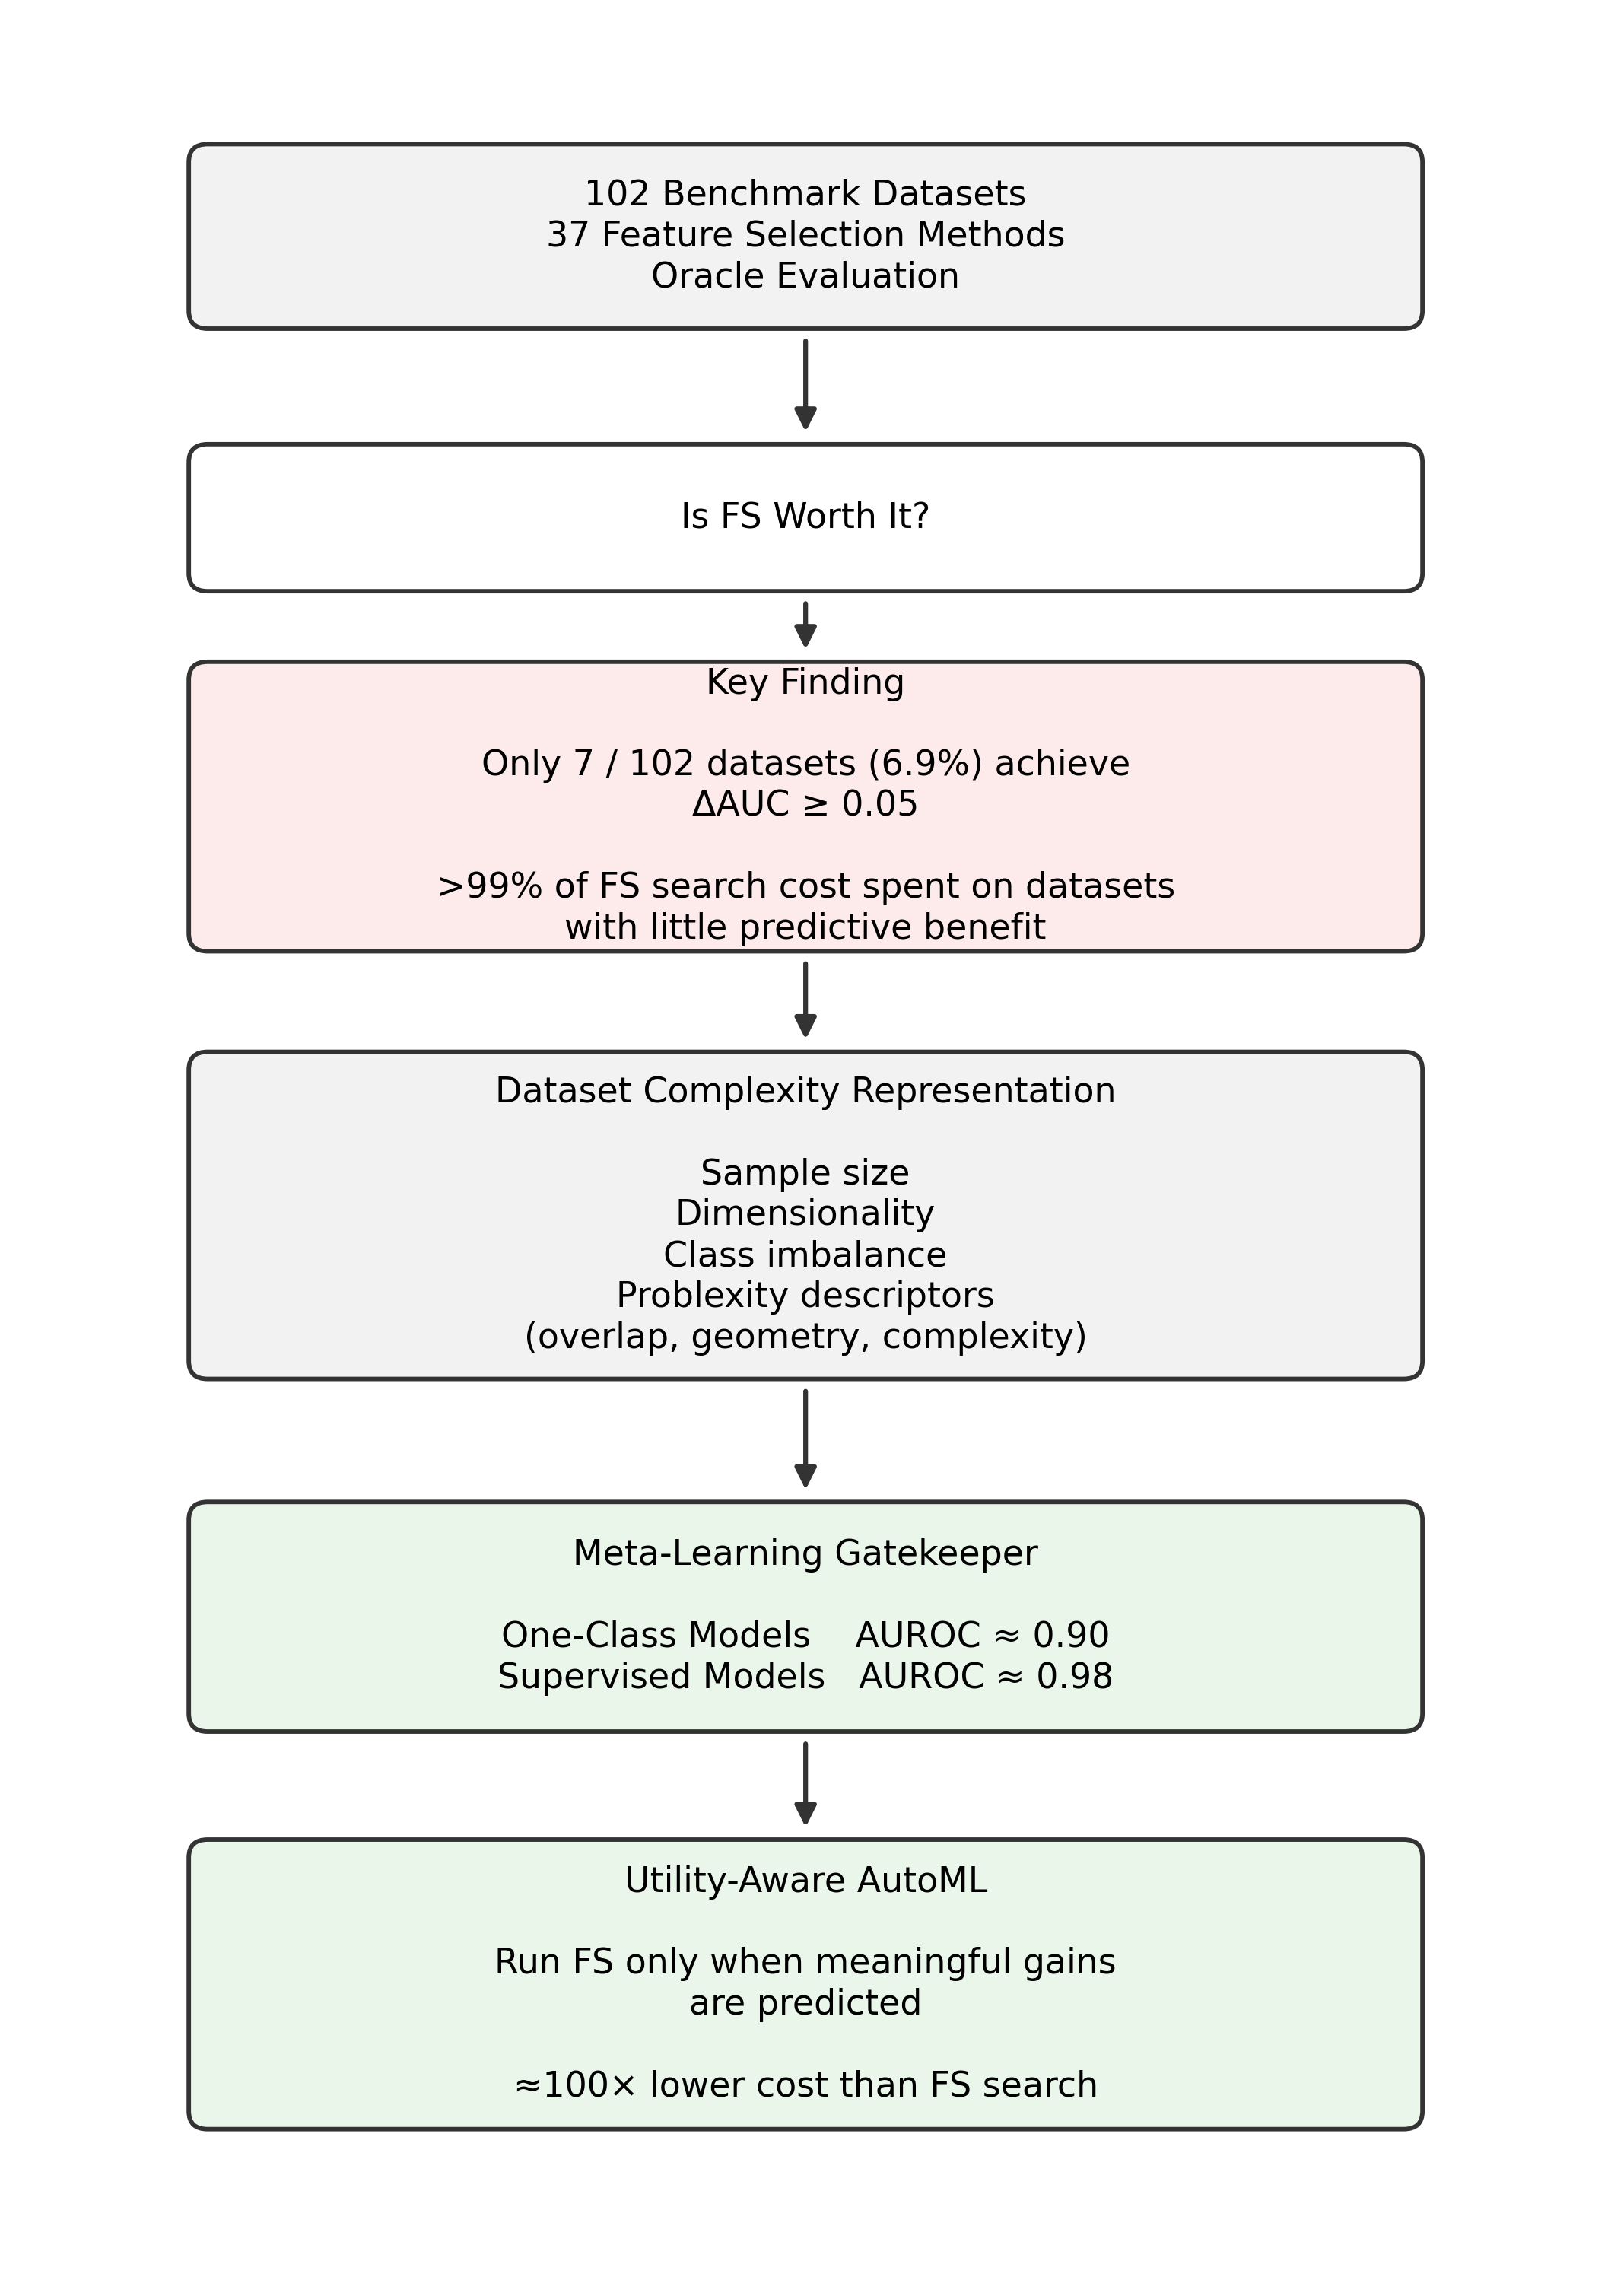
\includegraphics[height=0.82\textheight,keepaspectratio]{assets/graphical_abstract_vertical.png}
\end{graphicalabstract}

\begin{highlights}
\item Predicts when feature selection is likely to improve predictive performance
\item Oracle benchmark spans 37 FS algorithms across 102 classification datasets
\item Only 7 datasets achieve gains exceeding 0.05 AUC over the no-FS baseline
\item Feature-selection utility is predictable with high precision and recall
\item Utility is linked to class overlap, boundary complexity, and sample size
\end{highlights}

\begin{keyword}
Feature Selection \sep
Meta-Learning \sep
Algorithm Selection \sep
Dataset Complexity \sep
Anomaly Detection \sep
AutoML
\end{keyword}

\end{frontmatter}



\section{Introduction}
\label{sec:introduction}

Feature selection (FS) is routinely used in supervised learning pipelines under the assumption that removing irrelevant or redundant variables improves predictive performance. Consequently, most research in FS focuses on developing new selection algorithms or on recommending which algorithm to apply to a given dataset \citep{guyon2003introduction,li2017feature,jiao2023survey}. Implicit in this literature is a simple assumption: feature selection is generally beneficial for predictive performance.

A central finding of this work is that substantial predictive gains from feature selection are remarkably rare. Across 37 feature-selection algorithms and 102 datasets (Table \ref{tab:all_datasets}), we perform an oracle-style evaluation in which the best FS algorithm, classifier, and number of selected features are chosen independently for each dataset. Even under these highly favorable conditions, only 7 datasets achieve an AUC improvement of at least 0.05 points over the no-FS baseline (Table \ref{tab:auc_performance_all}). In other words, meaningful gains from feature selection occur in only 6.9\% of datasets.

More surprisingly, these 7 datasets account for less than 1\% of the total feature-selection search cost across the benchmark. The remaining 95 datasets consume more than 99\% of the computational effort while yielding no substantial predictive benefit. This reveals a striking mismatch between computational expenditure and predictive utility: feature selection is not only rarely beneficial, but the overwhelming majority of feature-selection computation is spent on datasets for which it provides little or no improvement in predictive performance.

This observation is consistent with a growing body of empirical work questioning the predictive utility of feature selection. Large-scale benchmarking studies have long emphasized the strong dataset dependence of FS performance and the absence of universally superior methods \citep{bommert2020benchmark,bommert2022benchmark}. More recently, several studies have challenged the assumption that sophisticated FS procedures consistently improve predictive performance. \cite{chen2026insignificance} showed that small random subsets of features often match or exceed carefully selected feature sets in high-dimensional datasets, particularly in gene-expression settings. Similarly, \cite{rajabinasab2026worse} demonstrated that many state-of-the-art unsupervised FS methods fail to outperform random feature selection, raising questions about the practical value added by increasingly complex selection procedures. Performance-driven benchmarks for modern tabular learning further show that FS effectiveness depends strongly on dataset characteristics and downstream learners \citep{cherepanova2023performance}. These studies establish that FS benefits are neither automatic nor universal. Our findings go one step further: not only are substantial gains rare, but the computational burden of feature selection is concentrated almost entirely on datasets that do not benefit from it.

This perspective exposes a gap in the current literature. Existing meta-learning and algorithm recommendation systems use dataset meta-features to recommend feature-selection algorithms \citep{parmezan2017metalearning,filchenkov2015datasets,shilbayeh2014feature}. However, these approaches generally assume that FS should be performed and therefore do not explicitly model the possibility that the optimal decision may be to avoid FS altogether.

The central objective of this paper is to determine whether the utility of feature selection itself is predictable. Rather than asking which FS algorithm to apply, we investigate whether a dataset is likely to benefit from feature selection before any FS algorithm is executed.

Our focus is deliberately narrow. Feature selection may be valuable for many reasons unrelated to predictive performance, including interpretability, scientific discovery, dimensionality reduction, fairness, privacy, explainability, and computational efficiency. These are important motivations and often justify the use of FS independently of any change in predictive accuracy. In this work, however, we focus exclusively on predictive performance. Specifically, we study whether a dataset is likely to achieve a meaningful improvement in downstream classification AUC after applying feature selection.

To investigate this hypothesis, we characterize datasets using both conventional meta-features and complexity descriptors. The meta-features include sample count, dimensionality, class imbalance, and feature-to-sample ratio. In addition, we employ complexity measures from the Problexity framework \citep{Komorniczak2023Problexity}, including N3 and F1. These features allow us to study whether datasets that benefit from FS occupy a distinct and identifiable region of dataset space.

The contribution of this paper is not a new FS algorithm. Instead, we formulate and study a previously overlooked prediction problem: estimating the utility of feature selection itself. By shifting the focus from algorithm recommendation to utility prediction, we seek to identify when feature selection is likely to improve predictive performance before any search is performed. This perspective is motivated not only by the rarity of substantial FS gains but also by the observation that the overwhelming majority of feature-selection computation is currently spent on datasets that derive no meaningful predictive benefit. Our goal is therefore to provide a principled framework for deciding when to attempt feature selection.

\paragraph{Key Findings}
Three main findings emerge. First, datasets that benefit substantially from feature selection are not randomly distributed throughout the benchmark corpus. They occupy a distinct region of the meta-feature space characterized by small sample sizes, greater class overlap, and more complex decision-boundary geometry. This indicates that the feature-selection utility is associated with identifiable structural properties of the learning problem.

Second, the feature-selection utility can be predicted directly from the dataset characteristics. Even when formulated as a rare-event detection problem, one-class models achieve strong discrimination between utility-beneficial and utility-neutral datasets, demonstrating that substantial gains from feature selection leave a detectable geometric signature.

Third, utility prediction becomes even more accurate when weak utility signals are incorporated into a supervised learning framework. Models trained on datasets exhibiting only modest feature-selection gains successfully generalize to datasets with substantially larger gains. This indicates that weak and strong FS-beneficial datasets share common structural characteristics, and that feature-selection utility follows a continuous and learnable structure rather than arising from isolated exceptional cases.


Finally, we show that utility prediction is computationally inexpensive relative to feature-selection search. Meta-feature extraction requires only a small fraction of the time needed for even a single feature-selection evaluation, while substantial feature-selection gains occur in only a small minority of datasets. This makes utility prediction a practical gatekeeper for avoiding unnecessary feature-selection searches.

\section{Related Work and Positioning}
\label{sec:related_work}

\subsection{Is Feature Selection Always Beneficial?}

Feature selection (FS) is one of the most widely used preprocessing techniques in machine learning. Classical studies motivate FS as a mechanism for removing irrelevant and redundant variables, improving predictive performance, reducing overfitting, and increasing model interpretability \citep{dash1997featureselection,kohavi1997wrappers,guyon2003introduction}. Consequently, a substantial portion of the FS literature focuses on developing new selection algorithms and demonstrating their effectiveness on benchmark datasets.

However, growing empirical evidence suggests that the predictive benefits of FS are far from universal. Large-scale benchmarking studies have repeatedly reported considerable variability in FS effectiveness across datasets, classifiers, and evaluation protocols \citep{bommert2020benchmark,bommert2022benchmark}. One of the earliest studies to investigate this question directly was conducted by \citet{post2016does}, who evaluated feature selection across nearly 400 OpenML datasets and 12 classification algorithms. Their results showed that FS improved predictive performance in only a subset of dataset–algorithm combinations and that statistically significant improvements were relatively uncommon. Importantly, they demonstrated that dataset characteristics such as dimensionality and task difficulty influence whether FS is beneficial.

More recent work has further challenged the assumption that sophisticated FS procedures consistently improve predictive performance. \citet{chen2025insignificance} showed that in many high-dimensional settings, carefully selected feature subsets often fail to outperform randomly chosen subsets. Similarly, \citet{rajabinasab2026worse} demonstrated that numerous modern unsupervised FS methods perform no better than random feature selection across a broad collection of benchmarks. Other domain-specific benchmarking studies have likewise reported that FS may provide little benefit or even degrade predictive performance depending on the classifier and dataset structure. Collectively, these findings suggest that FS should be viewed as a conditional operation whose utility depends strongly on the underlying characteristics of the learning problem.

\subsection{Meta-Learning for Feature Selection}

The observation that FS effectiveness varies across datasets naturally motivated the application of meta-learning techniques. Rather than seeking a universally optimal FS method, these approaches attempt to predict which FS algorithm is most appropriate for a new dataset based on dataset-level descriptors.

Several studies formulate FS recommendation as an algorithm-selection problem, using meta-features to map datasets to the most promising FS method \citep{parmezan2017metalearning,filchenkov2015datasets,shen2020metalearning}. More generally, this literature demonstrates that dataset characteristics can be exploited to guide preprocessing decisions and reduce the cost of exhaustive benchmarking.

Despite their success, most meta-learning approaches implicitly assume that some form of FS will ultimately be applied. Their objective is typically to determine \emph{which} FS method should be used rather than \emph{whether} FS should be performed at all. As a result, they operate downstream of the decision considered in the present work.

\subsection{Predicting Feature Selection Utility}

The work most closely related to ours is that of \citet{post2016does}, who explicitly investigated whether the benefit of feature selection can be predicted from dataset meta-features. Using a Random Forest meta-model, they predicted whether applying a specific FS method would improve the performance of a specific classifier on a given dataset. Their study established two important observations: FS utility is predictable from dataset descriptors, and FS effectiveness depends strongly on dataset characteristics.

Our work differs from this line of research in several important respects.

First, prior studies typically evaluate a single FS method or a small collection of methods and define utility as any positive performance improvement. In contrast, we adopt an oracle-style evaluation across 37 FS algorithms and multiple subset sizes, defining utility relative to the best achievable FS performance. This substantially reduces the risk that observed effects are artifacts of a particular selection method.

Second, we focus on \emph{practically meaningful} gains rather than arbitrary positive improvements. By introducing an operational threshold on $\Delta\mathrm{AUC}$, we distinguish datasets that derive substantial predictive benefit from FS from those exhibiting only negligible improvements. Under this formulation, genuinely beneficial datasets are rare, comprising only 7 of 102 benchmarks.

Third, we formulate utility prediction at the \emph{dataset level}. Existing work typically predicts whether a specific FS method improves a specific classifier on a specific dataset. Our objective is different: given a dataset, determine whether running an FS search is likely to be worthwhile before any FS algorithm is executed.

Fourth, we characterize utility through dataset complexity descriptors rather than relying primarily on conventional meta-features and landmarkers. Using Problexity measures and related geometric descriptors, we show that datasets benefiting from FS exhibit distinctive structural properties associated with class overlap, boundary complexity, and small-sample regimes.

Finally, our formulation leads to a substantially different learning problem. Under an oracle evaluation and a meaningful utility threshold, the population of datasets benefiting from FS becomes extremely small. This motivates treating utility prediction as a rare-event detection problem and enables a cost-aware analysis of when the computational expense of FS is justified.

\subsection{Positioning of the Present Work}

Prior work establishes two important facts. First, feature selection is not universally beneficial. Second, its effectiveness depends on measurable dataset characteristics. Existing research has therefore focused primarily on identifying the most suitable FS method for a given dataset or predicting whether a specific FS method will improve a specific classifier.

The present work addresses a different question. Rather than selecting among FS algorithms, we ask whether feature selection should be performed at all. Using an oracle evaluation spanning 37 FS algorithms, we show that substantial predictive gains from FS are exceptionally rare, occurring in only 6.9\% of benchmark datasets. We further demonstrate that these rare beneficial cases exhibit distinctive complexity profiles, can be identified accurately from dataset-level descriptors, and account for only a small fraction of the computational effort expended by exhaustive FS searches. This shifts the focus of meta-learning from algorithm recommendation to utility prediction and provides a practical framework for deciding whether to perform feature selection before the search process begins.



\section{Methodology}
\label{sec:methodology}

Our objective is to determine whether the predictive utility of feature selection can be estimated directly from dataset characteristics before feature selection is executed. We formulate this as a dataset-level prediction problem. Given a dataset and a collection of descriptive meta-features, the goal is to predict whether feature selection is likely to yield a meaningful improvement in downstream predictive performance.

The methodology consists of four components. First, we define a quantitative measure of feature-selection utility. Second, we represent each dataset using statistical and complexity-based meta-features. Third, we evaluate two predictive formulations: one-class rare-event detection and two-class supervised learning. Finally, we assess these predictions using both conventional predictive metrics and a decision-theoretic framework that quantifies the tradeoff between predictive benefit and computational cost.

\subsection{Defining Feature-Selection Utility}
\label{sec:utility_definition}

Let $\mathcal{D}_i$ denote the $i$-th dataset in the benchmark corpus. 
We define the best achievable performance under feature selection as

\begin{equation}
\mathrm{AUC}^{FS}(\mathcal{D}_i)
=
\max_{\substack{
a \in \mathcal{A} \\
K \in \mathcal{K} \\
c \in \mathcal{C}
}}
\mathrm{AUC}_{a,K,c}(\mathcal{D}_i).
\end{equation}


where $\mathcal{A}$ denotes the set of feature-selection algorithms, $\mathcal{K}$ the set of evaluated feature-subset sizes, and $\mathcal{C}$ the set of downstream classifiers.

Similarly, the best achievable performance without feature selection is

\begin{equation}
\mathrm{AUC}^{NoFS}(\mathcal{D}_i)
=
\max_{c \in \mathcal{C}}
\mathrm{AUC}_{\emptyset,c}(\mathcal{D}_i).
\end{equation}

The utility of feature selection is then defined as

\begin{equation}
\Delta_{AUC}(\mathcal{D}_i)
=
\mathrm{AUC}^{FS}(\mathcal{D}_i)
-
\mathrm{AUC}^{NoFS}(\mathcal{D}_i).
\label{eq:delta_auc}
\end{equation}

Positive values indicate that feature selection improves predictive performance, whereas values near zero indicate little practical benefit.

Importantly, in the present study, utility is defined purely in terms of the observed AUC difference and does not incorporate statistical significance testing. We intentionally adopt a more permissive criterion and consider any observed improvement above a threshold $\tau$ as potentially useful, regardless of whether the difference would be statistically significant under a formal hypothesis test. This choice operates in favour of feature selection: datasets exhibiting small, potentially non-significant improvements are still counted as benefiting from FS. Consequently, if substantial gains remain rare under this relaxed definition, the conclusion that feature-selection utility is uncommon is strengthened rather than weakened.


To convert utility into a prediction problem, we introduce a threshold parameter $\tau$. A dataset is considered feature-selection beneficial whenever

\begin{equation}
\Delta{AUC}(\mathcal{D}_i) \ge \tau.
\label{eq:tau_definition}
\end{equation}

Rather than committing to a single operating point, we evaluate multiple thresholds,

\begin{equation}
\tau \in {0.02, 0.03, 0.05, 0.08},
\end{equation}

allowing us to distinguish between modest improvements and substantial practical gains while assessing the robustness of our conclusions. For each threshold, datasets are relabeled according to Equation~\eqref{eq:tau_definition}, and the complete evaluation procedure is repeated.


\begin{table}[htbp]
\centering
\caption{Dataset-level descriptors used throughout the study. In addition to standard dataset meta-features, the representation includes 21 data-complexity measures from the Problexity framework \citep{Komorniczak2023Problexity}, which characterize feature overlap, class separability, decision-boundary complexity, neighborhood structure, topology, dimensionality, and class imbalance.}\label{tab:metafeatures}
\begin{tabular}{ll}
\toprule
Category & Features \\
\midrule
Basic meta-features &
$N$, $P$, $P/N$, $\log N$, $\log P$, is\_binary, Probe\_AUC\_0 \\
Feature overlap &
$f_1$, $f_{1v}$, $f_2$, $f_3$, $f_4$ \\
Linearity &
$l_1$, $l_2$, $l_3$ \\
Neighborhood &
$n_1$, $n_2$, $n_3$, $n_4$, LSC \\
Network topology &
density, clsCoef, hubs \\
Dimensionality &
$t_2$, $t_3$, $t_4$ \\
Class imbalance &
$c_1$, $c_2$ \\
\bottomrule
\end{tabular}
\end{table}

\subsection{Dataset Representation}
\label{sec:dataset_representation}

Each dataset is represented by a vector of dataset-level descriptors computed before any feature selection. The complete set of meta-features is summarized in Table~\ref{tab:metafeatures}.

The representation combines standard dataset descriptors with complexity measures derived from the Problexity framework \citep{Komorniczak2023Problexity}. The standard descriptors characterize basic properties of the learning problem, including sample size ($N$), dimensionality ($P$), feature-to-sample ratio ($P/N$), logarithmic transformations of dataset size ($\log N$, $\log P$), and class structure. We also include $\mathrm{Probe\_AUC}_0$, defined as the AUC of a baseline classifier trained on the original feature space without feature selection. This probe captures the dataset's baseline learnability and the available predictive headroom prior to applying FS.

To capture the geometric structure of the classification problem, we additionally compute 21 Problexity measures spanning feature overlap, class separability, linearity, neighborhood structure, network topology, dimensionality, and class imbalance. These include measures such as Fisher’s discriminant ratio ($f_1$), nearest-neighbor error ($n_3$), boundary non-linearity ($l_3$), local set cardinality (LSC), topological dimensionality measures ($t_2$–$t_4$), and class-imbalance descriptors ($c_1$, $c_2$). Together, these descriptors provide a compact characterization of dataset geometry and classification difficulty.

The primary predictive models use only intrinsic dataset descriptors and do not incorporate domain metadata. This design choice is deliberate. Several datasets exhibiting substantial feature-selection gains originate from similar application domains, particularly genomics, and including domain labels would risk learning dataset provenance rather than intrinsic properties of the learning problem. Domain metadata is therefore reserved exclusively for ablation analyses, where it is used to test whether the utility of feature selection is better explained by dataset geometry or dataset provenance.



\subsection{Utility Prediction Models}
\label{sec:prediction_models}

We evaluate two formulations of the utility-prediction problem.

The first formulation treats FS-beneficial datasets as rare events. In this setting, the model is trained on the dominant No-FS population and assigns an anomaly or rarity score to each dataset. We evaluate a diverse set of rare-event models spanning reconstruction-based, density-based, isolation-based, and boundary-based approaches: PCA reconstruction, shallow autoencoders, Local Outlier Factor, Isolation Forest, and One-Class SVM. The shallow autoencoder is included as a high-capacity reference model. Given the limited number of datasets, we do not expect neural representation learning to be advantageous; instead, the comparison tests whether the signal governing FS utility is better captured by simple low-dimensional structure.

The second formulation treats FS utility as a supervised two-class prediction problem. Because the strongly beneficial class at $\tau=0.05$ is too small to train on directly, we use weakly beneficial datasets as positive training examples. Specifically, we define $P_{0.01}$ as the set of datasets satisfying $\Delta_{AUC} \ge 0.01$ and $P_{0.05}$ as the set satisfying $\Delta_{AUC} \ge 0.05$. The supervised training positives are then $P_{\mathrm{weak}} = P_{0.01} \setminus P_{0.05}$. 

The strongly beneficial datasets in $P_{0.05}$ are excluded from training and reserved for testing. We evaluate Logistic Regression, Random Forest, and XGBoost under this formulation. For each model family, we train an ensemble of 50 models. Each ensemble member uses the same weak-positive datasets and a different randomly sampled set of negative datasets of equal size. This produces balanced training sets while reducing sensitivity to the particular negative sample.



\subsection{Feature Selection Pipeline}

Our FS pipeline follows the principles introduced in \cite{elmakias2025choosing}, but is adapted to assess FS algorithms rather than dataset difficulty. For each dataset, we evaluate FS in a downstream classification setting using five common classifiers: Logistic Regression (LR), Support Vector Machine with RBF kernel (SVM), Random Forest (RF), Extremely Randomized Trees (ET), and XGBoost.

Each FS algorithm is applied within a stratified 5-fold cross-validation framework. In every fold:
\begin{enumerate}
    \item The training split is used to fit the FS algorithm.
    \item A subset of $K$ features is selected, with $K \in \{1,5,30,60\}$.
    \item The same selected features are applied to the held-out test split.
    \item Each classifier is trained on the selected training features and evaluated on the selected test features.
    \item Runtime of the FS step only and predictive performance are recorded.
\end{enumerate}

The selected values of $K$ are intended to cover a practical range from very sparse selections ($K=1,5$) to moderate-dimensional subsets ($K=30,60$), while keeping the search space feasible across 37 algorithms, 102 datasets, and multiple classifiers. For datasets with fewer than $K$ available features, the maximum feasible number of features is used. The no FS pipeline is the same as $K=p$ (the total number of features).

Importantly, feature selection itself is always fitted only on the training split of each fold. The \emph{Oracle} setting is not a nested-validation estimate of deployment performance; rather, it is a post-hoc benchmark summary used to estimate the potential value of systematic configuration search. We therefore interpret \emph{Oracle} as an upper-bound, not as an unbiased estimate of what a fully nested model-selection pipeline would achieve on a new dataset.



\subsection{Evaluation Protocol}
\label{sec:evaluation_protocol}

The rare-event and supervised formulations are evaluated using different protocols because they answer different statistical questions.

For rare-event models, we use repeated balanced subsampling. At each repetition, the model is trained exclusively on datasets from the \textsc{No-FS} population; feature-selection-beneficial datasets are never used during training. The test set contains all feature-selection-beneficial datasets at the chosen threshold and an equal number of randomly sampled \textsc{No-FS} datasets. At $\tau=0.05$, this yields a balanced test set with seven positive and seven negative datasets. The negative test sample is redrawn $50$ times, and performance is summarized across repetitions. This protocol avoids evaluating AUROC on a single positive example and reduces sensitivity to the particular choice of negative test datasets.

For supervised models, training is repeated across $50$ balanced resampling iterations. In each iteration, all weak-positive datasets ($P_{0.01} \setminus P_{0.05}$) are included in the training set, together with a randomly sampled set of negative datasets of equal size. The strong-positive datasets in $P_{0.05}$ are excluded from training and are used only for evaluation. The test set in each iteration consists of all datasets in $P_{0.05}$ together with seven randomly sampled datasets satisfying $\Delta_{\mathrm{AUC}} < 0.01$. This yields $50$ supervised training/evaluation episodes and reduces dependence on a single arbitrary choice of negative test examples.

Performance is evaluated using AUROC, accuracy, precision, recall, F1 score, and balanced accuracy. Unless otherwise stated, binary predictions are obtained by thresholding model scores at $0.5$ for supervised models and by using the predefined anomaly-score threshold for rare-event models. Reported results are summarized across the $50$ balanced repetitions using the median and interquartile range, with bootstrap confidence intervals reported where appropriate. Recall is particularly important because failing to identify a genuinely feature-selection-beneficial dataset directly sacrifices attainable predictive performance.

\section{Results}
\label{sec:results}

We first examine whether datasets that benefit substantially from feature selection occupy a distinct region of the meta-feature space. We then evaluate utility prediction as a rare-event detection problem using one-class models, before testing whether weak utility signals can be used to train supervised predictors that yield stronger feature-selection benefits. Finally, we quantify the computational overhead of extracting the dataset descriptors used by the utility predictors. Detailed characteristics of all 102 benchmark datasets are presented in Table~\ref{tab:all_datasets} (Appendix), and the corresponding predictive performance obtained with and without feature selection is reported in Table~\ref{tab:auc_performance_all} (Appendix).

All experiments were conducted on a high-performance compute environment comprising (i)~10$\times$ NVIDIA RTX A5000 GPUs, (ii)~512~GB RAM, and (iii)~2$\times$ AMD EPYC 7443 CPUs (24 cores each).



\subsection{Datasets Benefiting from Feature Selection Are Structurally Distinct}
\label{sec:results_geometry}

Figure~\ref{fig:delta_auc_histogram} shows the distribution of feature-selection utility across the benchmark. Consistent with the motivating observation of Section~\ref{sec:introduction}, substantial gains are rare. Only seven datasets achieve improvements exceeding the operational threshold $\tau = 0.05$, while the overwhelming majority cluster around $\Delta\mathrm{AUC}=0$.

\begin{figure}[htbp]
\centering
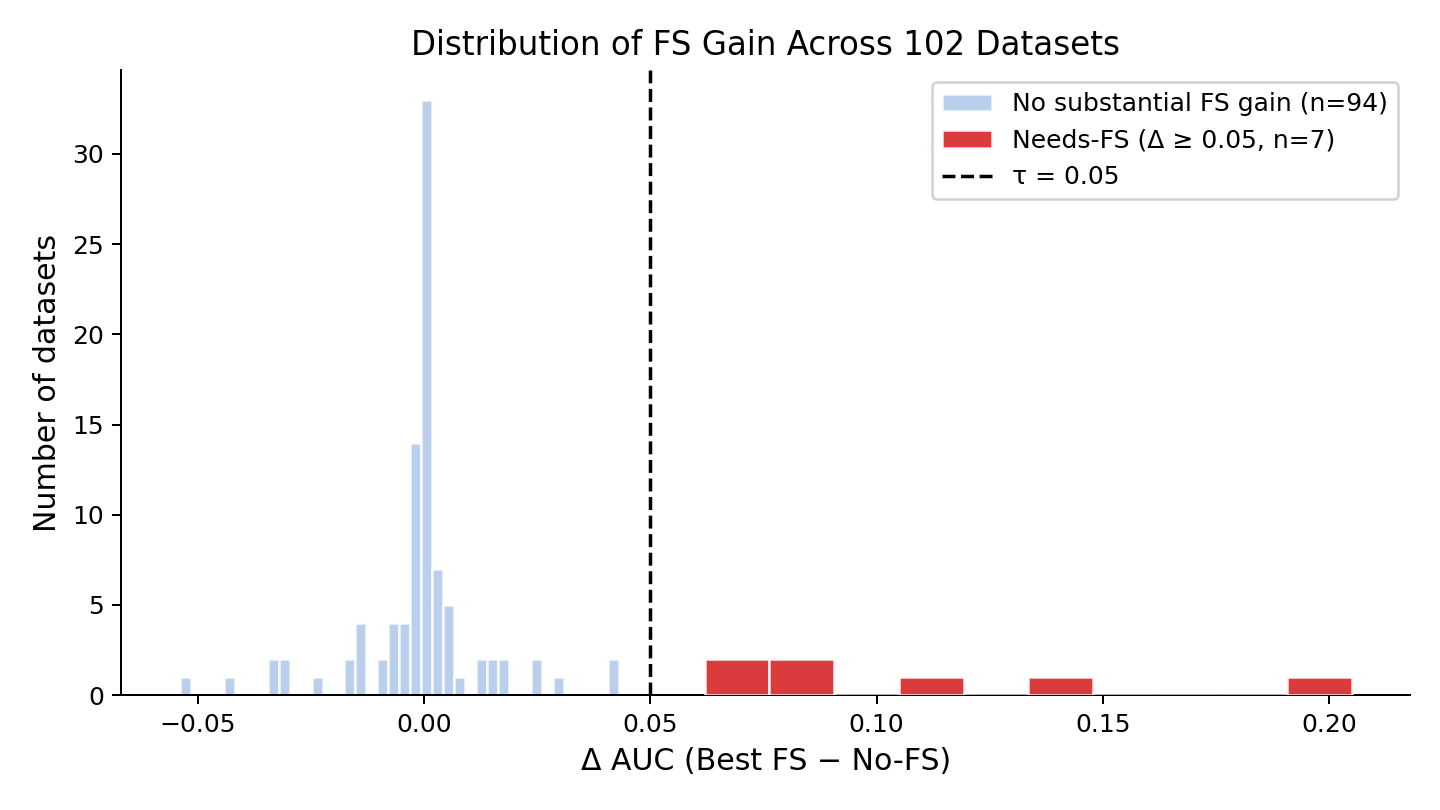
\includegraphics[width=0.75\textwidth]{assets/delta_auc_histogram.png}
\caption{Distribution of feature-selection utility across the benchmark datasets. The dashed vertical line denotes the operational threshold $\tau=0.05$ used to define the \textsc{Needs-FS} class.}
\label{fig:delta_auc_histogram}
\end{figure}

The central question is therefore whether these seven datasets are structurally distinguishable from the remaining benchmark problems. To address this, we performed a univariate effect-size analysis over the dataset meta-features. For each meta-feature, datasets were partitioned into the \textsc{Needs-FS} group ($\Delta\mathrm{AUC} \geq 0.05$) and the \textsc{No-FS} group ($\Delta\mathrm{AUC} < 0.05$). We report Cohen’s $d$ for continuity with the main analysis and Hedges’ $g$ as a small-sample corrected standardized effect size. Unlike predictive feature-importance measures such as permutation importance or SHAP values, these effect sizes do not measure a feature’s contribution inside a trained model. They measure only the degree to which a single meta-feature separates the two populations. We complement the effect-size analysis with Mann–Whitney U tests and Benjamini–Hochberg correction across the tested meta-features. Given the small number of \textsc{Needs-FS} datasets, these statistics should be interpreted as evidence of benchmark-level separation rather than as definitive population-level estimates.

Figure~\ref{fig:effect_sizes} summarizes the strongest univariate differences. The largest corrected effects are observed for $\mathrm{Probe_AUC}_0$ (Hedges’ $g=-3.31$, BH-adjusted $p=0.0014$), followed by $t_3$ ($g=1.16$), $n_3$ ($g=0.97$), $f_1$ ($g=0.93$), and $\log N$ ($g=-0.83$). After Benjamini–Hochberg correction, $\mathrm{Probe_AUC}_0$ remains significant, while the other geometric descriptors retain large descriptive effects but do not survive correction at $q<0.05$.

The direction of these effects is informative. The negative effect for $\mathrm{Probe_AUC}_0$ indicates that \textsc{Needs-FS} datasets have substantially lower baseline performance before feature selection, suggesting greater predictive headroom. The negative effect for $\log N$ indicates that they also tend to be smaller. In contrast, the positive effects for $t_3$, $n_3$, and $f_1$ indicate greater classification difficulty, class overlap, and boundary complexity. Together, these results suggest that feature-selection utility is associated with low baseline separability and difficult class geometry rather than with dimensionality alone.

Importantly, the dominant effects are not simply raw dimensionality descriptors. Rather, the strongest differences involve baseline learnability, class overlap, neighborhood structure, and boundary geometry. This supports the central hypothesis that feature-selection utility is linked to the structure of the learning problem, not merely to the number of features.

\begin{figure}[htbp]
\centering
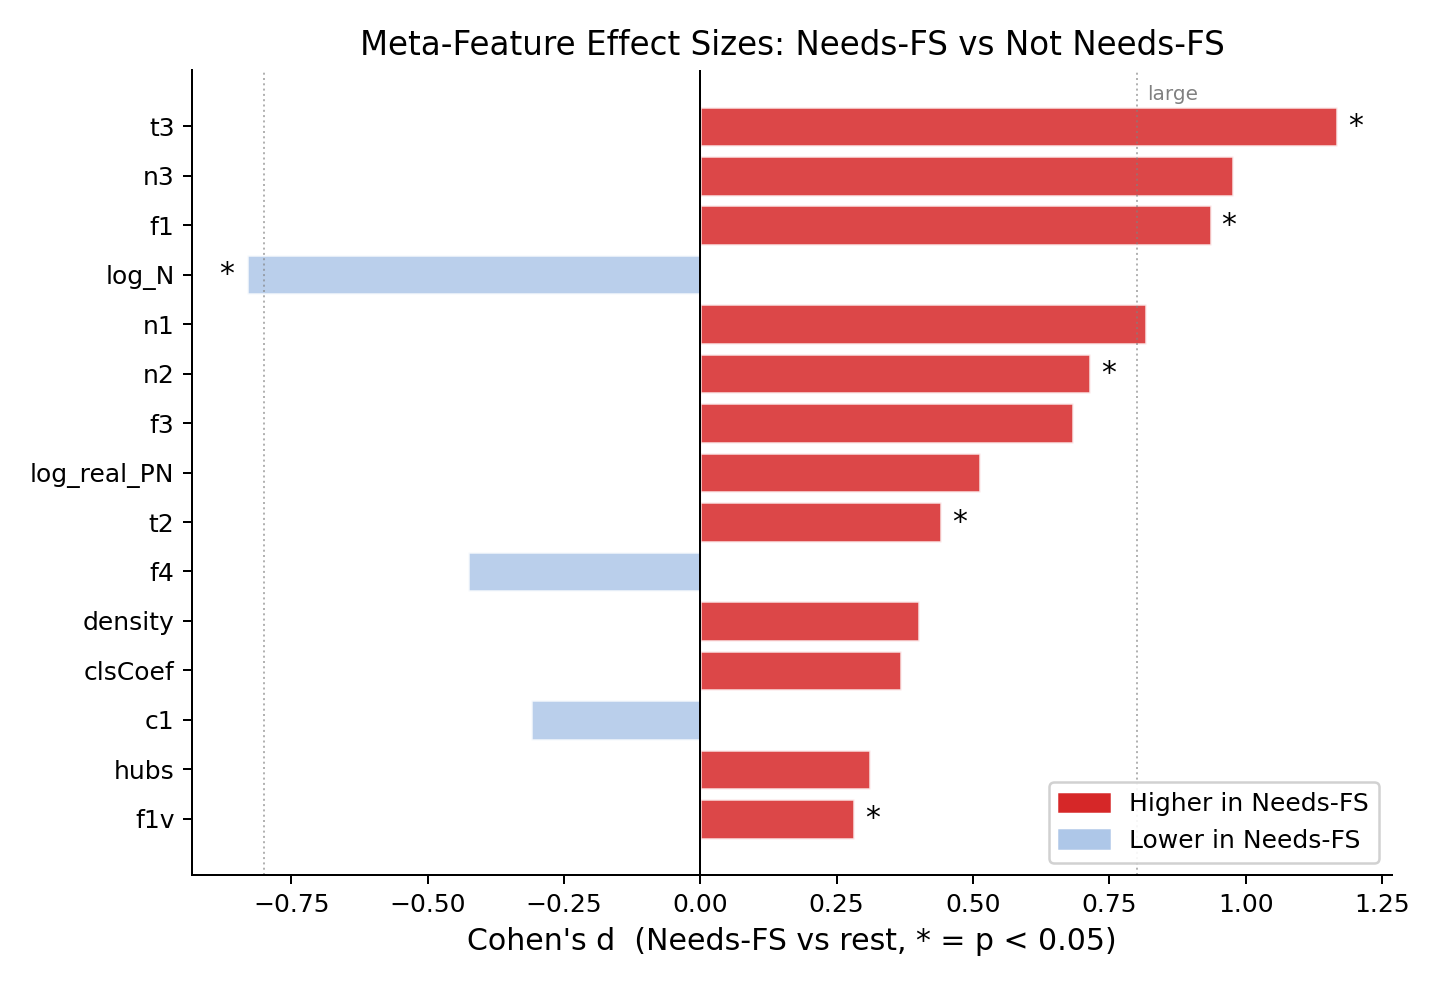
\includegraphics[width=0.85\textwidth]{assets/top_feature_effect_sizes.png}
\caption{Meta-feature effect sizes comparing \textsc{Needs-FS} and \textsc{No-FS} datasets. Bars show Cohen’s $d$, with positive values indicating larger values among datasets benefiting from feature selection. In the revised robustness analysis, Hedges’ $g$ and Benjamini–Hochberg adjusted $p$-values are also reported; $\mathrm{Probe_AUC}_0$ remains significant after correction.}
\label{fig:effect_sizes}
\end{figure}

We also examined whether the observed separation could be explained by benchmark provenance. No datasets from the Stiglic collection were present in the analyzed corpus, and none of the seven strong-positive datasets originate from that source. Thus, the separation reported above cannot be attributed to Stiglic-specific dependence among datasets. More generally, domain composition does not explain the positive class: genomic datasets account for $71%$ of the strong-positive group but also $75%$ of the negative group. Therefore, being genomic is not sufficient to explain feature-selection utility in this benchmark.

\subsection{One-Class Utility Prediction}
\label{sec:results_oneclass}

We next evaluate whether feature-selection utility can be detected without using positive examples during training. Following the protocol of Section~\ref{sec:evaluation_protocol}, rare-event models are trained exclusively on the dominant \textsc{No-FS} population and evaluated using repeated balanced subsampling. At $\tau=0.05$, each evaluation set contains all seven \textsc{Needs-FS} datasets and seven randomly sampled \textsc{No-FS} datasets.

Table~\ref{tab:oneclass_results} and Figure~\ref{fig:ad_auroc_curves} summarize the one-class results. All methods outperform random guessing, indicating that datasets benefiting from feature selection are not arbitrary outliers but occupy a detectable region of the meta-feature space. Autoencoder reconstruction achieves the highest median AUROC ($0.898$), while PCA reconstruction and OC-SVM closely follow ($0.888$). PCA reconstruction provides the best balance between precision and recall, achieving median precision, recall, F1, and accuracy of $0.857$. In contrast, Isolation Forest obtains the weakest recall ($0.286$), suggesting that its isolation-based inductive bias is less well matched to this rare-event structure.

\begin{table}[htbp]
\centering
\footnotesize
\caption{Performance of one-class utility prediction models at $\tau=0.05$. Training is performed exclusively on \textsc{No-FS} datasets, while evaluation uses balanced test sets containing all seven \textsc{Needs-FS} datasets and seven randomly sampled \textsc{No-FS} datasets. Values report median performance across $50$ repeated balanced-subsampling trials, with IQR in parentheses.}
\label{tab:oneclass_results}
\begin{tabular}{lccccc}
\toprule
Model & AUROC & Precision & Recall & F1 & Accuracy \\
\midrule
Autoencoder        & 0.90 (0.12) & 0.83 (0.29) & 0.71 (0.14) & 0.80 (0.08) & 0.79 (0.13) \\
PCA Reconstruction & 0.89 (0.12) & 0.86 (0.25) & 0.86 (0.00) & 0.86 (0.12) & 0.86 (0.14) \\
OC-SVM             & 0.89 (0.12) & 0.75 (0.08) & 0.86 (0.00) & 0.80 (0.05) & 0.79 (0.07) \\
LOF                & 0.87 (0.14) & 0.83 (0.29) & 0.71 (0.00) & 0.77 (0.12) & 0.79 (0.14) \\
Isolation Forest   & 0.80 (0.16) & 0.67 (0.41) & 0.29 (0.00) & 0.40 (0.04) & 0.57 (0.07) \\
\bottomrule
\end{tabular}
\end{table}

The threshold sweep in Figure~\ref{fig:ad_auroc_curves} provides additional insight. Lower thresholds include a broader set of weak-gain datasets, whereas higher thresholds isolate the smaller group of datasets with substantial FS gains. As $\tau$ increases, most detectors improve, suggesting that the strongest \textsc{Needs-FS} datasets form a more coherent and identifiable subgroup than the broader weak-gain population. Across most thresholds, PCA reconstruction is among the most stable one-class methods, making it a useful baseline for detecting feature-selection-beneficial datasets from intrinsic descriptors alone.

\begin{figure}[htbp]
\centering
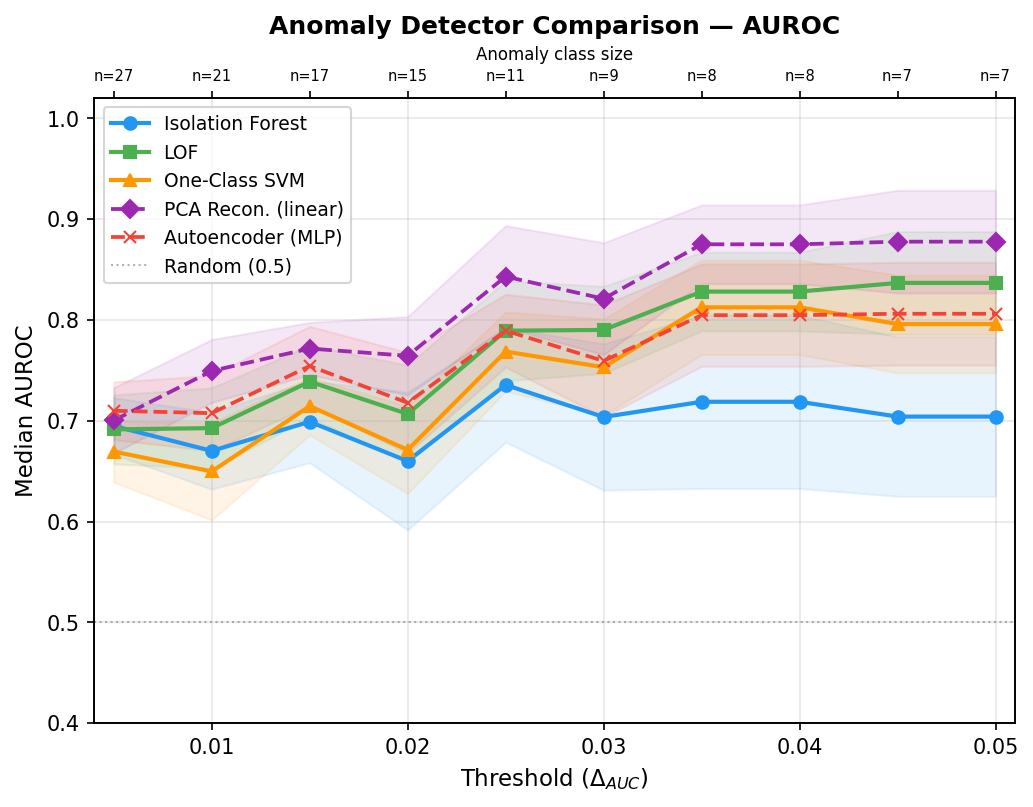
\includegraphics[width=0.85\textwidth]{assets/ad_auroc_curves.png}
\caption{Median AUROC of five rare-event detectors as a function of the operating threshold $\tau \in [0.005,0.05]$, evaluated under the Problexity representation. Shaded regions indicate $\pm 1$ standard-deviation intervals over $R=50$ balanced subsampling repetitions. The number of feature-selection-beneficial datasets at each threshold is shown along the top axis.}
\label{fig:ad_auroc_curves}
\end{figure}

\subsection{Supervised Utility Prediction Using Weak Positives}
\label{sec:results_supervised}

The one-class results show that utility prediction is feasible even without positive training examples. We next ask whether weaker utility signals can be used to train supervised predictors of stronger FS benefit. For each operating threshold $\tau$, datasets with gains below $\tau$ but above a weaker lower threshold are treated as weak positives during training, while the datasets satisfying the stronger threshold are held out for evaluation. This design tests whether modest and substantial FS gains share a common structural signature.

Figure~\ref{fig:twoclass_auroc_vs_tau} summarizes the supervised results across operating thresholds. All three supervised models perform well above random guessing throughout the threshold range. Logistic Regression is consistently competitive with, and often superior to, the tree-based alternatives. This suggests that the separation between utility-beneficial and utility-neutral datasets is captured by a relatively low-dimensional and approximately linear structure in the meta-feature space.

\begin{figure}[htbp]
\centering
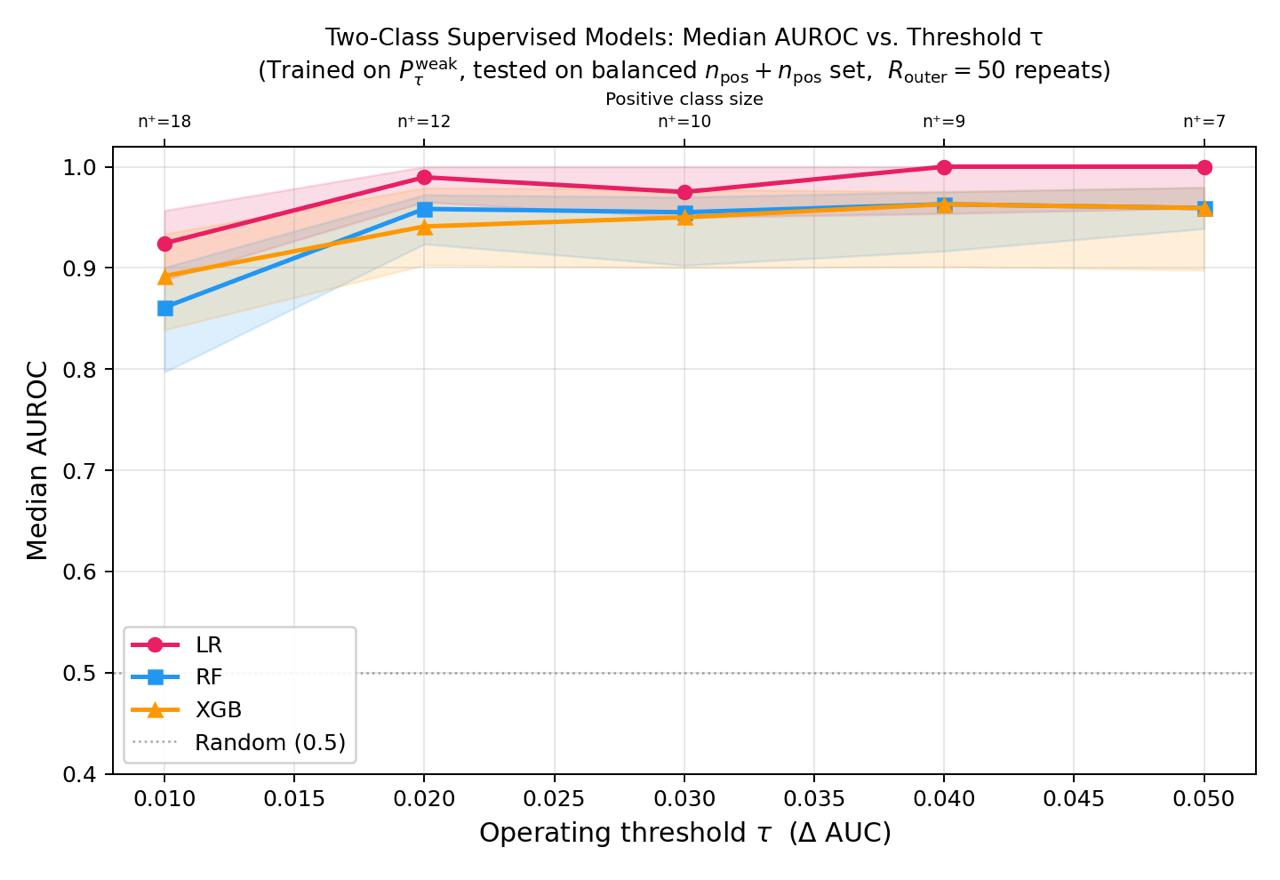
\includegraphics[width=0.85\textwidth]{assets/twoclass_auroc_vs_tau.jpeg}
\caption{Median AUROC of the two-class supervised utility predictors as a function of the operating threshold $\tau$. Models are trained on weak-positive datasets and evaluated on balanced test sets containing all strong positives at the corresponding threshold and an equal number of randomly sampled negatives. Shaded regions indicate variability over $R=50$ repeated negative-sampling evaluations.}
\label{fig:twoclass_auroc_vs_tau}
\end{figure}

Table~\ref{tab:supervised_results} reports the detailed supervised performance at the primary threshold $\tau=0.05$. The seven strong-positive datasets are fixed across evaluations, while the negative test examples are resampled. Logistic Regression achieves perfect median separation on the balanced benchmark evaluation sets, with median and AUROC equal to $1.000$. This result is not perfectly stable across all repetitions: the mean AUROC is $0.980$ with standard deviation $0.031$, and the bootstrap confidence interval for the median AUROC is $[0.980,1.000]$. Thus, the appropriate interpretation is not that the model is universally perfect, but that the strong-positive datasets are highly separable in the benchmark meta-feature space.

Random Forest and XGBoost also perform strongly, each achieving median AUROC of $0.959$. All three models maintain high recall, with median recall of $1.000$. This is important because failing to identify a genuinely FS-beneficial dataset forfeits attainable predictive gain.

\begin{table}[htbp]
\centering
\footnotesize
\caption{Supervised utility prediction using weak positives at $\tau=0.05$. Models are trained on weak-positive datasets and evaluated on balanced test sets containing all seven strong positives and seven randomly sampled negatives. Values report medians across $50$ repeated negative-sampling evaluations, with IQR in parentheses.}
\label{tab:supervised_results}
\begin{tabular}{lccccc}
\toprule
Model & AUROC & Accuracy & Precision & Recall & F1 \\
\midrule
LR      & 1.00 (0.04) & 0.86 (0.07) & 0.78 (0.10) & 1.00 (0.00) & 0.88 (0.06) \\
RF      & 0.96 (0.04) & 0.86 (0.07) & 0.78 (0.16) & 1.00 (0.14) & 0.86 (0.08) \\
XGBoost & 0.96 (0.08) & 0.86 (0.14) & 0.78 (0.18) & 1.00 (0.00) & 0.88 (0.11) \\
\bottomrule
\end{tabular}
\end{table}
These results strengthen the conclusion drawn from the one-class experiments. The positive datasets are not merely detectable as outliers from the \textsc{No-FS} population; their structure is sufficiently coherent that weak positives can be used to learn a supervised decision rule that transfers to stronger positives. This supports the view that feature-selection utility is not an isolated property of a few exceptional datasets, but rather follows a continuous and learnable structure in dataset space.

At the same time, the size of the strong-positive class imposes an important limitation. At $\tau=0.05$, the evaluation involves only seven \textsc{Needs-FS} datasets. The supervised results should therefore be interpreted as evidence of strong separability within this benchmark, rather than as a definitive estimate of population-level predictive performance.

\subsection{Geometry, Not Provenance, Drives Utility Prediction}
\label{sec:results_ablation}

A natural concern is that the supervised models may learn dataset provenance rather than intrinsic structure. To test this, we compared three feature representations: intrinsic descriptors only, domain/provenance features only, and their combination. The intrinsic representation includes the basic meta-features and complexity descriptors used throughout the paper, while the domain representation consists only of repository and category indicators.

Table~\ref{tab:feature_set_ablation} shows that provenance alone is not predictive of feature-selection utility. The domain-only representation obtains median AUROC of $0.281$, far below the intrinsic representation. In contrast, the intrinsic representation achieves median and AUROC of $1.000$. Adding domain metadata to the intrinsic descriptors does not improve performance and slightly reduces the median AUROC to $0.998$. These results indicate that the utility predictor is not simply memorizing the dataset source or domain membership. Instead, the predictive signal is carried primarily by the intrinsic properties of the learning problem.

% \begin{table}[htbp]
% \centering
% \caption{Feature-set ablation for supervised utility prediction at $\tau=0.05$. Values report medians across $50$ repeated evaluations, with IQR in parentheses.}
% \label{tab:feature_set_ablation}
% \begin{tabular}{lcccc}
% \toprule
% Feature set & AUROC & Precision & Recall & F1 \\
% \midrule
% Intrinsic descriptors    & 1.000 (0.000) & 1.000 (0.000) & 0.857 (0.143) & 0.923 (0.090) \\
% Domain/provenance only   & 0.281 (0.041) & 0.000 (0.000) & 0.000 (0.000) & 0.000 (0.000) \\
% Combined                 & 0.998 (0.003) & 1.000 (0.000) & 0.429 (0.000) & 0.600 (0.000) \\
% \bottomrule
% \end{tabular}
% \end{table}

\begin{table}[htbp]
\centering
\footnotesize
\caption{Feature-set ablation for supervised utility prediction at $\tau=0.05$. Values report medians across $50$ repeated evaluations, with IQR in parentheses.}
\label{tab:feature_set_ablation}
\begin{tabular}{lcccc}
\toprule
Feature set & AUROC & Precision & Recall & F1 \\
\midrule
Intrinsic descriptors  & 1.00 (0.00) & 1.00 (0.00) & 0.86 (0.14) & 0.92 (0.09) \\
Domain/provenance only & 0.28 (0.04) & 0.00 (0.00) & 0.00 (0.00) & 0.00 (0.00) \\
Combined               & 1.00 (0.00) & 1.00 (0.00) & 0.43 (0.00) & 0.60 (0.00) \\
\bottomrule
\end{tabular}
\end{table}

This finding also addresses the concern that the model may simply be identifying genomic datasets. Although five of the seven strong-positive datasets are genomic, genomic datasets are similarly prevalent in the negative class: they constitute 71\% of the strong-positive group and 75\% of the negative group. Domain membership, therefore, cannot explain the observed separation. 


\subsection{Computational Overhead of Utility Prediction}
\label{sec:results_overhead}

A natural concern is that computing dataset descriptors introduces additional preprocessing cost. We therefore measured the wall-clock time required to extract the complete meta-feature representation and compared it with the cost of feature-selection evaluation. Figure~\ref{fig:gatekeeper_vs_fs_boxplot} shows the aggregate comparison. Across the matched benchmark datasets, meta-feature extraction required a median of only $7.99$ seconds, whereas a single feature-selection algorithm evaluated at a single subset size required a median of $972.8$ seconds. Thus, even before accounting for the fact that a full FS search evaluates many algorithms and subset sizes, the ratio of median costs is approximately $122\times$ in favor of the utility-prediction stage.

\begin{figure}[htbp]
\centering
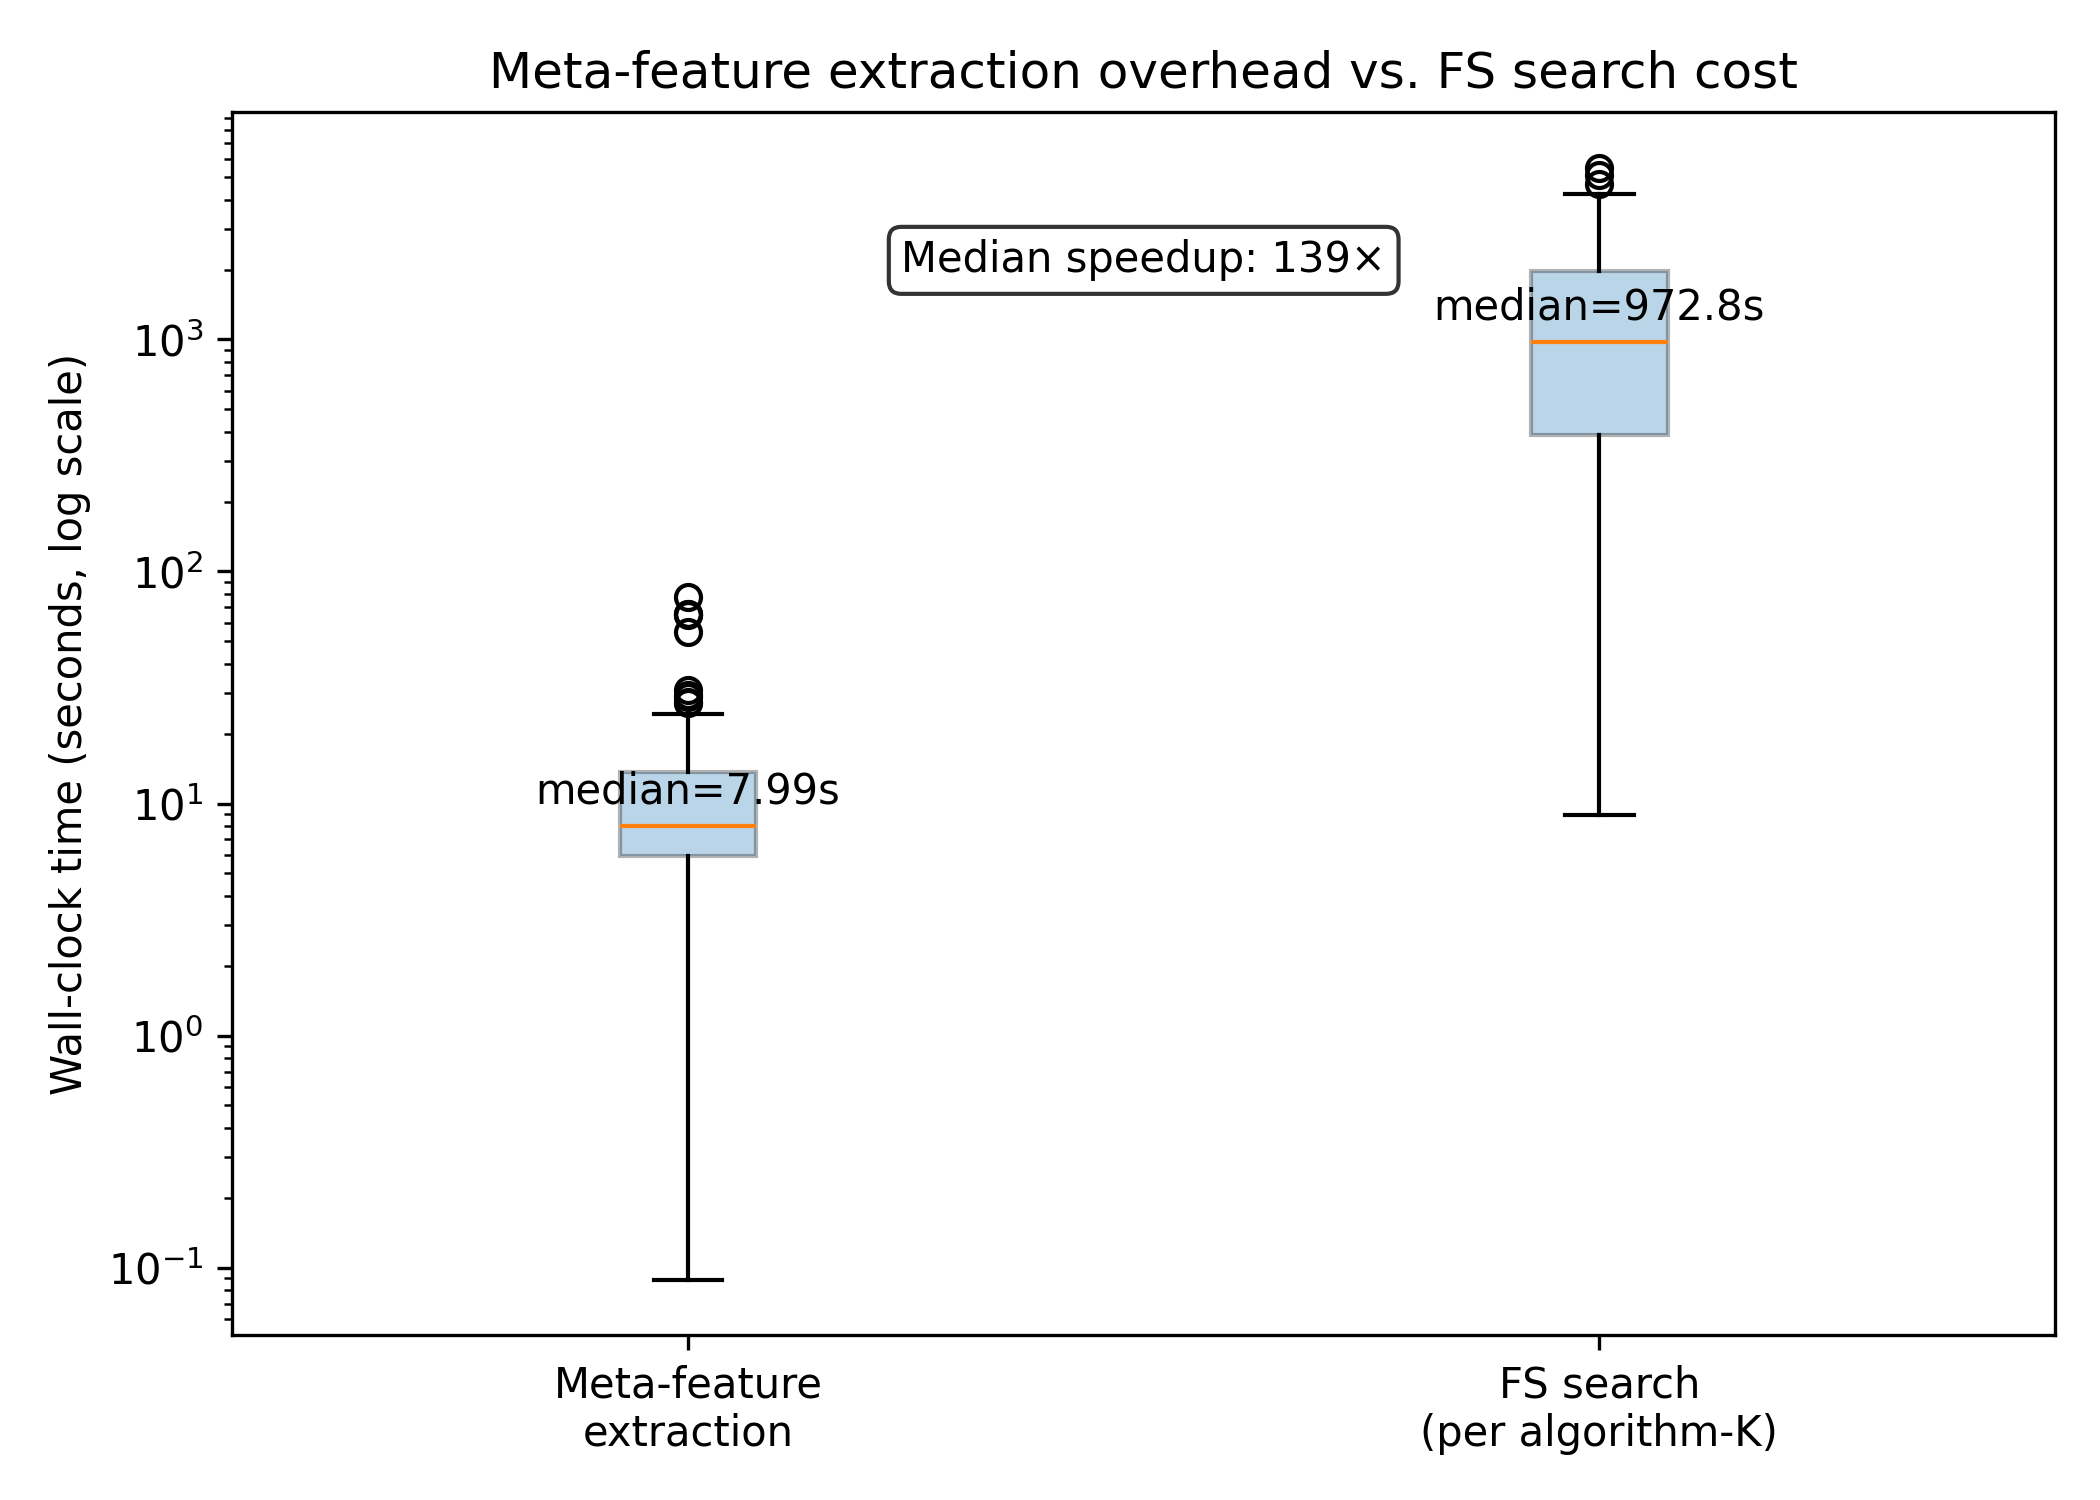
\includegraphics[width=0.75\textwidth]{assets/gatekeeper_vs_fs_boxplot.png}
\caption{Aggregate computational cost of meta-feature extraction versus a single feature-selection evaluation. Times are shown on a logarithmic scale. Meta-feature extraction is computed once per dataset, whereas each FS observation corresponds to one dataset, one FS algorithm, and one subset size.}
\label{fig:gatekeeper_vs_fs_boxplot}
\end{figure}

Figure~\ref{fig:gatekeeper_overhead_vs_fs_scatter} shows the same comparison at the dataset level. Each point corresponds to one dataset. The $x$-axis reports the one-time cost of extracting the meta-feature representation, while the $y$-axis reports the average runtime of a single FS evaluation on that dataset, averaged over all evaluated FS algorithms and subset sizes. The comparison is therefore conservative: the plotted FS cost corresponds to one average selector configuration rather than the full cost of searching over the complete FS algorithm–$K$ grid. All datasets lie above the break-even line, and the majority lie above the $10\times$ and $100\times$ reference lines.

\begin{figure}[htbp]
\centering
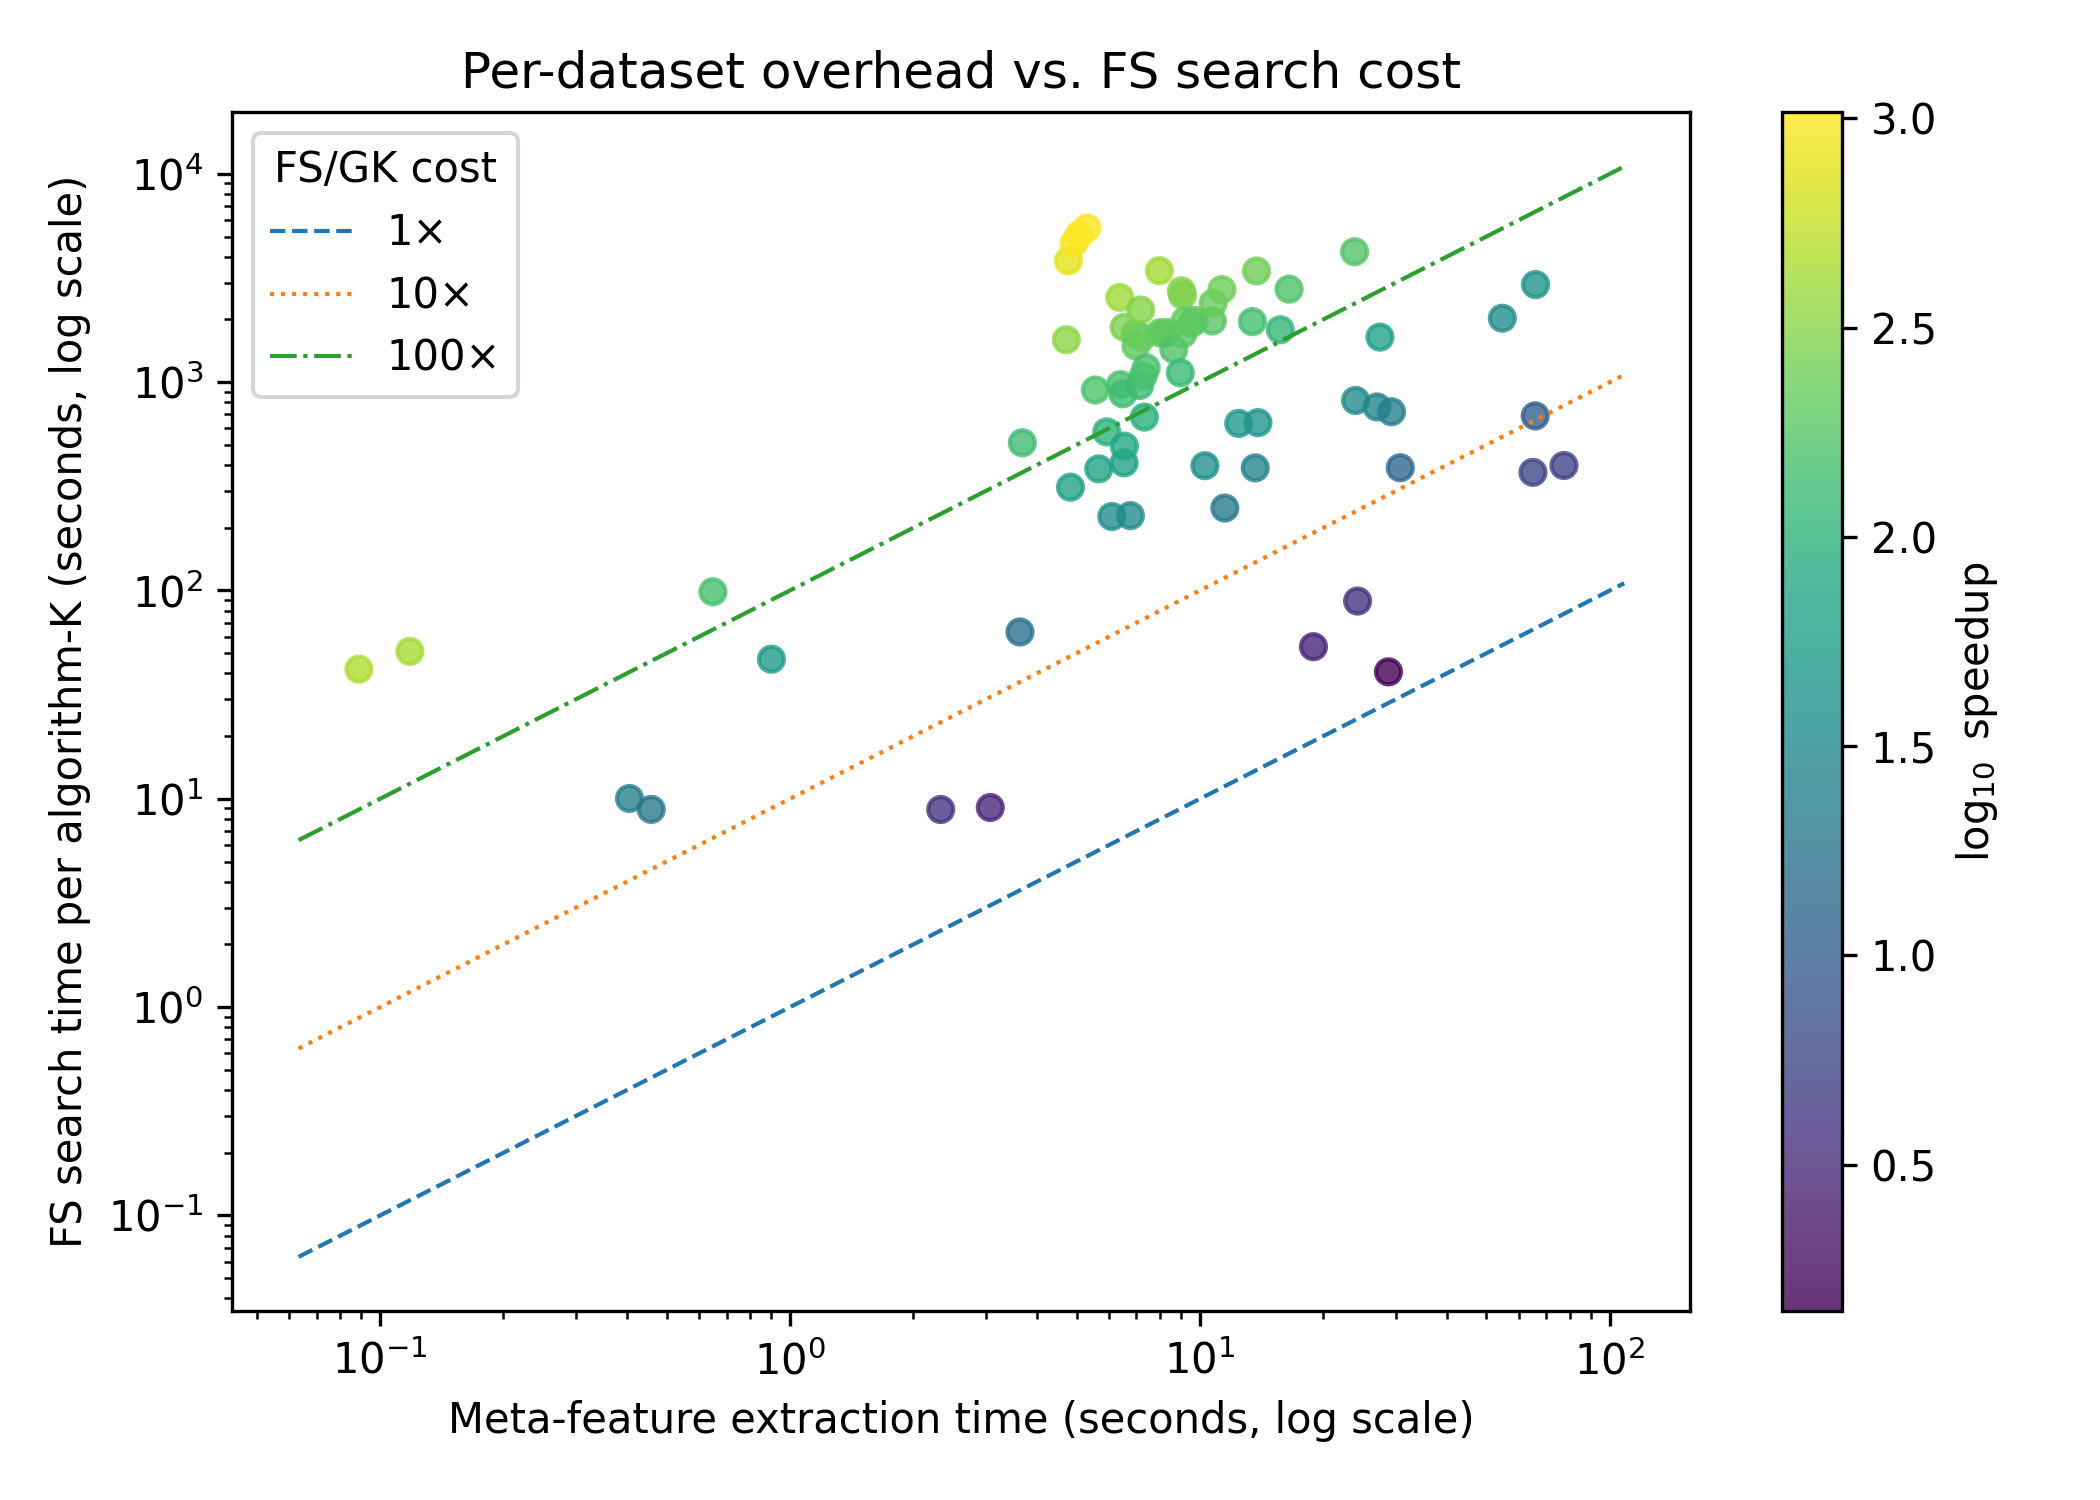
\includegraphics[width=0.78\textwidth]{assets/gatekeeper_overhead_vs_fs_scatter.png}
\caption{Per-dataset comparison between meta-feature extraction overhead and feature-selection evaluation cost. Both axes are logarithmic. Diagonal reference lines indicate equal cost, $10\times$ speedup, and $100\times$ speedup.}
\label{fig:gatekeeper_overhead_vs_fs_scatter}
\end{figure}

Figure~\ref{fig:gatekeeper_speedup_ecdf} summarizes the distribution of per-dataset speedups, defined as the ratio between FS evaluation time and meta-feature extraction time. The median per-dataset speedup is $139\times$, and no dataset in the matched benchmark has a meta-feature extraction cost exceeding the average single FS evaluation cost. These results show that the proposed utility-prediction step is not an expensive substitute for FS search, but rather a lightweight diagnostic stage whose computational cost is typically one to two orders of magnitude smaller than that of a single FS evaluation.

\begin{figure}[htbp]
\centering
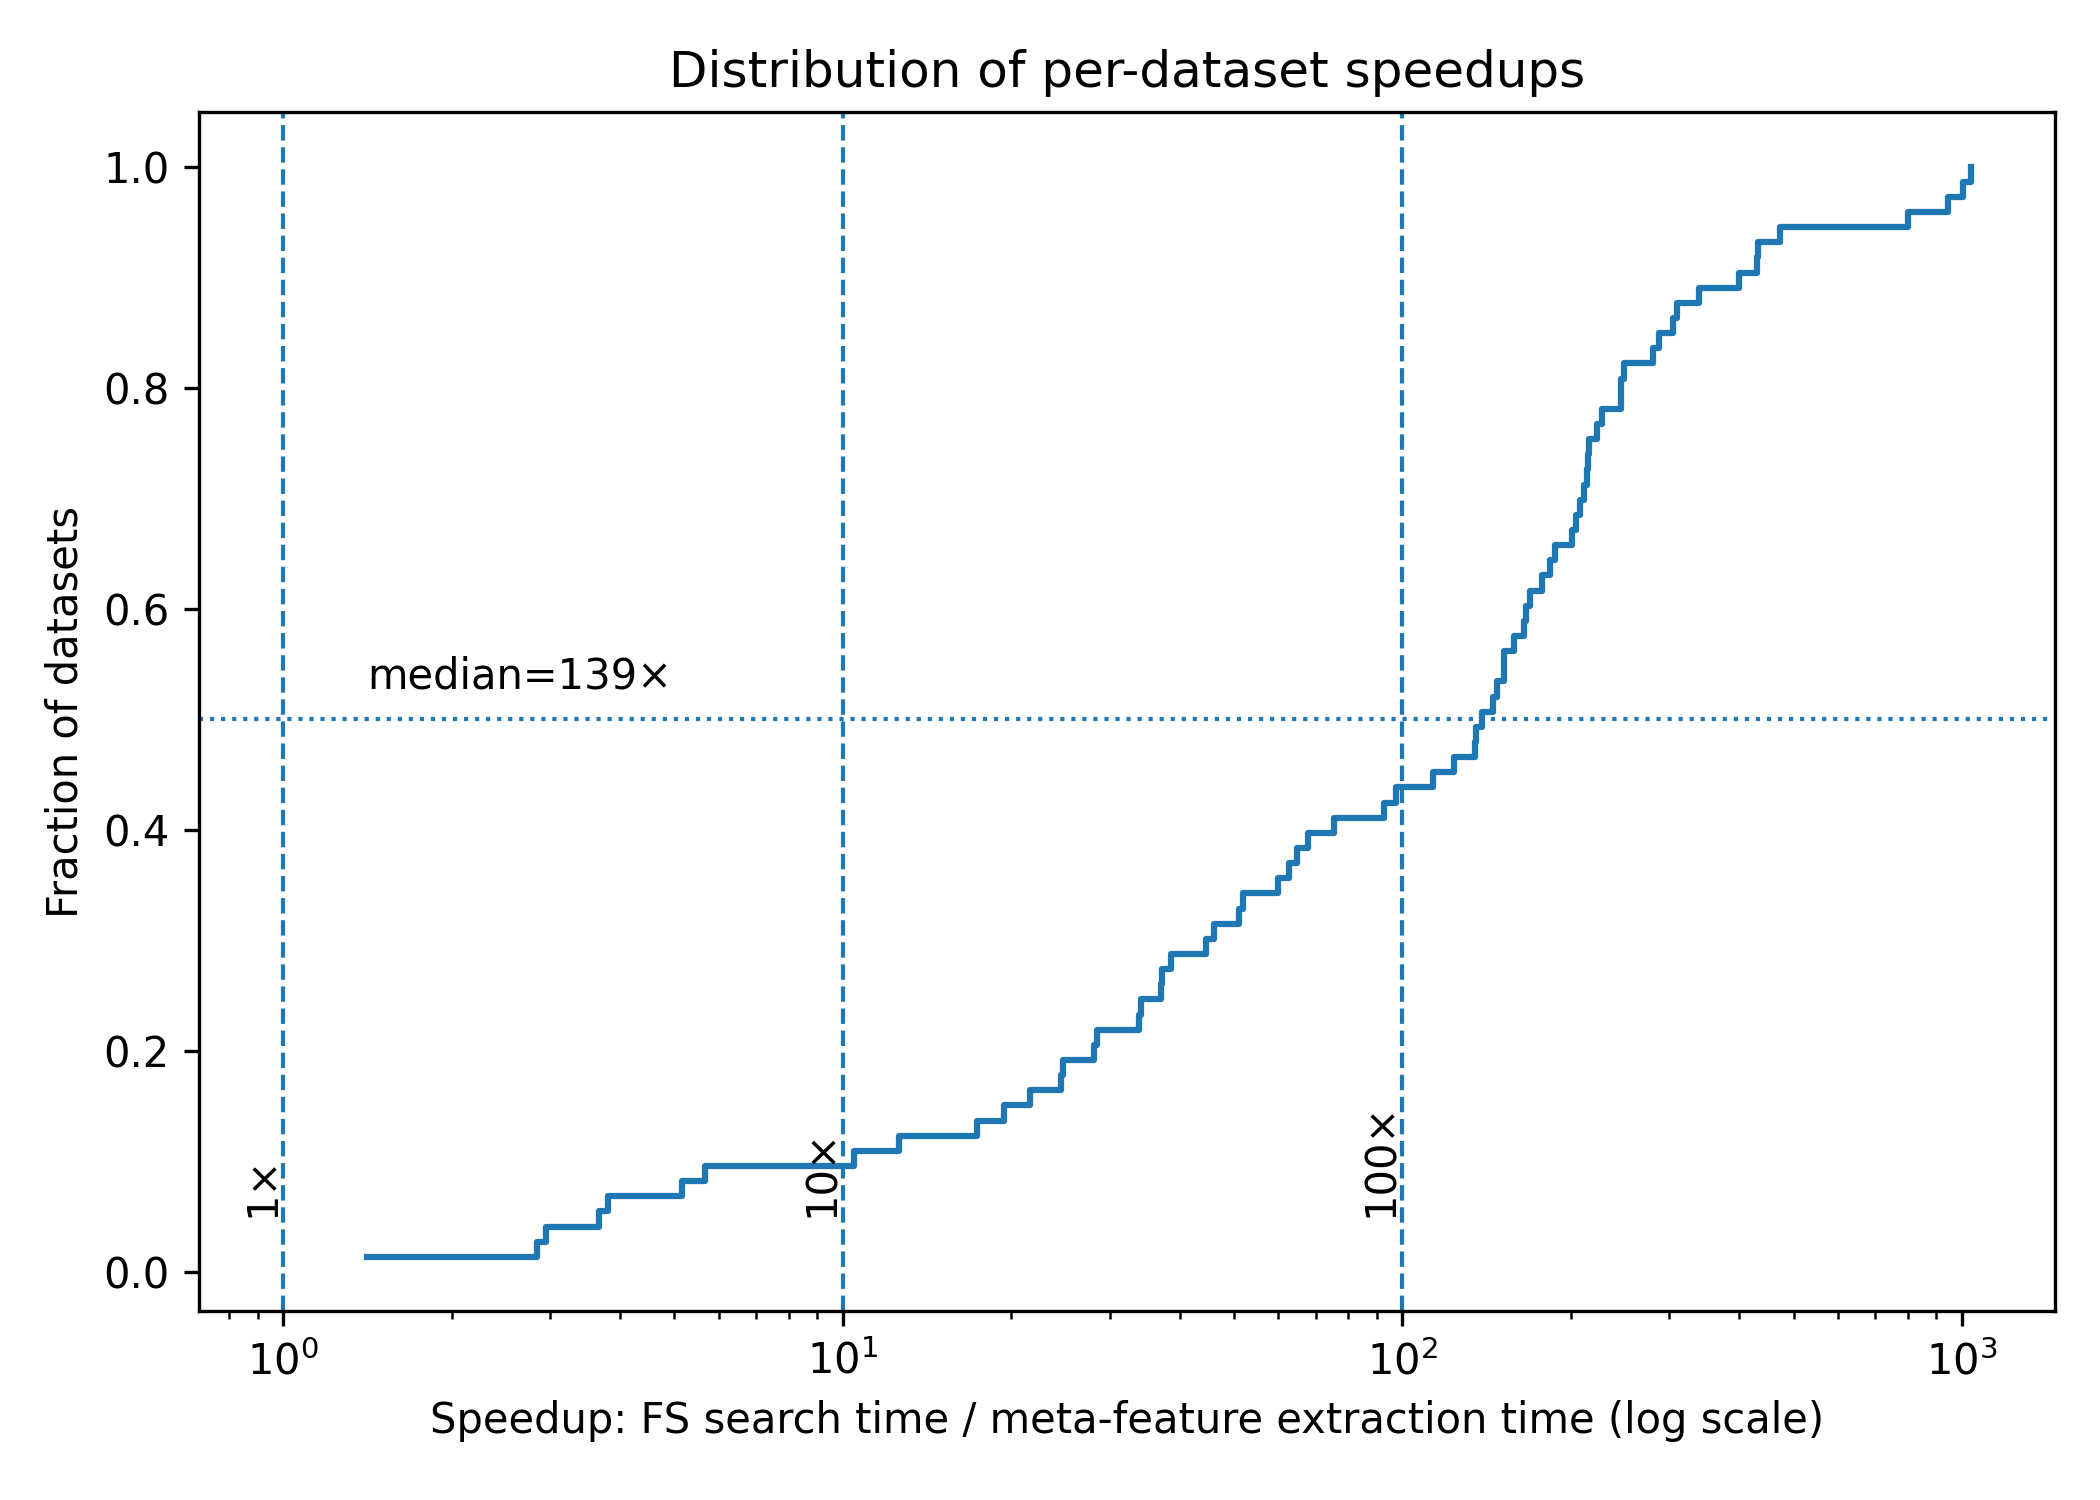
\includegraphics[width=0.75\textwidth]{assets/gatekeeper_speedup_ecdf.png}
\caption{Empirical cumulative distribution of per-dataset speedups, defined as FS evaluation time divided by meta-feature extraction time. Vertical reference lines indicate $1\times$, $10\times$, and $100\times$ speedup.}
\label{fig:gatekeeper_speedup_ecdf}
\end{figure}

Finally, our benchmark includes both lightweight filter methods and more expensive wrapper, embedded, and neural-network-based approaches. We intentionally compare meta-feature extraction against the cost of the broader feature-selection search process rather than only against the cost of the cheapest individual FS method. In practice, once a practitioner decides that FS is warranted, the relevant question is often not whether to run a single inexpensive selector, but which method and subset size achieve the best trade-off between predictive performance and computational cost. Evaluating only a lightweight filter may provide some improvement, but it does not reveal whether substantially larger gains are attainable from more expressive or computationally intensive selectors.



\section{Discussion and Conclusions}
\label{sec:conclusion}

Feature selection is commonly treated as a standard preprocessing step in machine-learning pipelines. In this paper, we revisited this assumption by asking a more fundamental question: can the utility of feature selection itself be predicted before any feature-selection algorithm is executed?

Using an oracle-style evaluation spanning 37 feature-selection algorithms across 102 benchmark datasets, we found that substantial predictive gains from feature selection are remarkably rare. Only seven datasets achieved an improvement of at least 0.05 AUC over the no-feature-selection baseline, corresponding to approximately 6.9\% of the benchmark corpus. Moreover, these seven datasets accounted for less than 1\% of the total feature-selection search cost, while the overwhelming majority of computational effort was spent on datasets that derived little or no predictive benefit.

We showed that datasets benefiting from feature selection are not randomly distributed throughout the benchmark collection. Instead, they exhibit distinctive structural characteristics, including lower baseline predictive performance, smaller sample sizes, greater class overlap, and more complex decision-boundary geometry. These differences are captured by dataset-level complexity descriptors and can be detected without executing any feature-selection procedure.

Building on this observation, we formulated feature-selection utility prediction as both a rare-event detection problem and a supervised learning problem. One-class models achieved strong discrimination between utility-beneficial and utility-neutral datasets, while supervised models trained only on weakly beneficial datasets generalized successfully to the held-out datasets exhibiting the largest gains. Taken together, these results demonstrate that feature-selection utility is not merely observable retrospectively but is predictable from intrinsic dataset properties.

An important question is whether the observed predictive performance reflects genuine structural regularities or simply memorization of dataset provenance. Several robustness analyses support the former interpretation. A domain-only baseline using repository and dataset-category indicators achieved a median AUROC of only 0.281, substantially below random performance, whereas the intrinsic complexity representation achieved a median AUROC of 1.000. Combining domain and complexity information produced no meaningful improvement over complexity descriptors alone. These results indicate that the predictive signal arises primarily from the geometry of the learning problem rather than from benchmark-specific identifiers or source collections.

A related concern is that the positive class may simply reflect particular application domains, such as high-dimensional genomic datasets. However, domain composition analysis does not support this explanation. Genomic datasets constitute approximately 71\% of the strong-positive class but also approximately 75\% of the negative class. Thus, domain membership alone cannot explain the observed separation. Instead, feature-selection utility appears to be associated with structural characteristics such as baseline separability, class overlap, neighborhood complexity, and decision-boundary geometry, irrespective of application domain.

From a practical perspective, these findings suggest a simple deployment strategy. Before initiating an expensive feature-selection search, a practitioner can first compute inexpensive dataset-level descriptors and estimate the probability that feature selection will provide meaningful predictive benefit. If the predicted utility is low, the computational cost of evaluating dozens of feature-selection algorithms and subset sizes may be avoided entirely. If the predicted utility is high, computational resources can be focused on the comparatively small subset of datasets where feature selection is most likely to improve performance. The computational-overhead analysis suggests that this screening stage is typically one to two orders of magnitude cheaper than the search procedures it is intended to replace.

The study has several limitations. First, the benchmark comprises 102 datasets, of which only seven satisfy the strongest utility criterion. Although this scarcity is itself a central empirical finding, it inevitably limits statistical power and increases uncertainty when estimating population-level performance. For example, the strongest supervised model achieved a median AUROC of 1.000, but the corresponding mean AUROC across repeated evaluations was 0.980, with a bootstrap confidence interval of [0.980, 1.000]. These results indicate strong separability within the benchmark while also highlighting the uncertainty inherent in evaluating extremely rare events. Second, utility was defined exclusively in terms of predictive-performance improvement. Feature selection may be valuable for many other reasons, including interpretability, scientific discovery, fairness, privacy, explainability, model compression, and regulatory requirements. These aspects were intentionally excluded from the present analysis. Third, the evaluation focuses exclusively on tabular classification problems and may not directly generalize to regression, time-series forecasting, graph learning, or deep representation learning settings.

Several directions for future work emerge naturally from these findings. First, larger and more diverse benchmark collections would allow a more comprehensive characterization of feature-selection utility across domains and learning paradigms. Second, future studies could investigate utility prediction under alternative objectives, including interpretability, sparsity, computational efficiency, fairness, and multi-objective optimization. Third, the strong performance of simple linear models suggests that feature-selection utility may possess a relatively low-dimensional structure that deserves further theoretical investigation. Finally, integrating utility prediction directly into AutoML systems could enable adaptive preprocessing pipelines that invoke feature selection only when dataset characteristics indicate that meaningful gains are likely.

More broadly, our results suggest a shift in perspective. Rather than treating feature selection as a default preprocessing operation, it may be more appropriate to view it as a costly intervention whose usefulness depends on the geometry and complexity of the underlying learning problem. Under this view, the central question is no longer which feature-selection algorithm to apply, but whether feature selection should be applied at all. Our results suggest that this decision can often be made accurately using inexpensive dataset-level descriptors, potentially avoiding substantial computational effort on datasets for which feature selection is unlikely to provide meaningful predictive benefit.


\appendix
{\footnotesize
\begin{longtable}{@{}r p{1.9cm} p{6.7cm} r r r r@{}}
\caption{All 102 datasets used in this study, sorted by descending feature-selection gain. \textbf{\#C}: number of classes (2 = binary); \textbf{$p$}: number of features; \textbf{$n$}: number of samples; \textbf{MAJ}: majority class proportion. Sorting follows descending $\Delta\mathrm{AUC}=\mathrm{FS\ AUC}-\mathrm{No\text{-}FS\ AUC}$; $\Delta\mathrm{AUC}$ is shown in the next table.}
\label{tab:all_datasets} \\
\toprule
\textbf{\#} & \textbf{Category} & \textbf{Dataset} & \textbf{\#C} & \textbf{$p$} & \textbf{$n$} & \textbf{MAJ} \\
\midrule
\endfirsthead
\multicolumn{7}{c}{{\bfseries \tablename\ \thetable{} -- continued from previous page}} \\
\toprule
\textbf{\#} & \textbf{Category} & \textbf{Dataset} & \textbf{\#C} & \textbf{$p$} & \textbf{$n$} & \textbf{MAJ} \\
\midrule
\endhead
\midrule
\multicolumn{7}{r}{{Continued on next page}} \\
\endfoot
\bottomrule
\endlastfoot

1 & Gene & colon, Alon \citeyearpar{alon1999broad} & 2 & 2000 & 62 & 65\% \\
2 & Biological & Period\_Changer, G{\"u}l \citeyearpar{period_changer_729} & 2 & 1177 & 90 & 70\% \\
3 & Gene & CNS, Pomeroy \citeyearpar{pomeroy2002prediction} & 2 & 7129 & 60 & 65\% \\
4 & Gene & tumors\_C, Pomeroy \citeyearpar{pomeroy2002prediction} & 2 & 7129 & 60 & 65\% \\
5 & Gene & ALLAML, Golub \citeyearpar{golub1999molecular} & 2 & 7129 & 72 & 65\% \\
6 & Other & madelon, Guyon \citeyearpar{guyon2004result} & 2 & 500 & 2600 & 50\% \\
7 & Chemical & Musk2, Chapman \citeyearpar{musk_(version_2)_75} & 2 & 166 & 6598 & 85\% \\
8 & Gene & Prostate-GE, Li \citeyearpar{li2017feature} & 2 & 5966 & 102 & 51\% \\
9 & Gene & CLL-SUB-111, Haslinger \citeyearpar{haslinger2004microarray} & 3 & 11340 & 111 & 46\% \\
10 & Gene & AP\_Omentum\_Ovary, Stiglic \citeyearpar{stiglic2010stability} & 2 & 10236 & 275 & 72\% \\
11 & Gene & nci9, Li \citeyearpar{li2017feature} & 9 & 9712 & 60 & 15\% \\
12 & Gene & Breast, Pochet \citeyearpar{pochet2004systematic} & 2 & 24481 & 97 & 53\% \\
13 & Gene & Brain1, Pomeroy \citeyearpar{pomeroy2002prediction} & 5 & 5920 & 90 & 67\% \\
14 & Gene & SMK-CAN-187, Li \citeyearpar{li2017feature} & 2 & 19993 & 187 & 52\% \\
15 & Healthcare & hepatitis, Hopkins \citeyearpar{hepatitis_46} & 2 & 19 & 154 & 55\% \\
16 & Biological & Bioresponse, Vanschoren \citeyearpar{vanschoren2014openml} & 2 & 1776 & 3751 & 54\% \\
17 & Chemical & glass, German \citeyearpar{glass_identification_42} & 7 & 9 & 213 & 36\% \\
18 & Gene & GCM, Ramaswamy \citeyearpar{ramaswamy2001multiclass} & 14 & 16063 & 190 & 16\% \\
19 & Imaging & warpAR10P, Li \citeyearpar{li2017feature} & 10 & 2400 & 130 & 10\% \\
20 & Gene & GLI-85, Freije \citeyearpar{freije2004gene} & 2 & 22283 & 85 & 69\% \\
21 & Text & spambase, Hopkins \citeyearpar{spambase_94} & 2 & 57 & 4600 & 60\% \\
22 & Gene & AP\_Ovary\_Uterus, Stiglic \citeyearpar{stiglic2010stability} & 2 & 10236 & 322 & 60\% \\
23 & Imaging & Yale, Li \citeyearpar{li2017feature} & 15 & 1024 & 165 & 7\% \\
24 & Chemical & biodegradation, Mansouri \citeyearpar{mansouri2013quantitative} & 2 & 41 & 1055 & 66\% \\
25 & Imaging & orlraws10P, Li \citeyearpar{li2017feature} & 10 & 10304 & 100 & 10\% \\
26 & Chemical & COIL20, Li \citeyearpar{li2017feature} & 20 & 1024 & 1440 & 5\% \\
27 & Gene & AP\_Breast\_Lung, Stiglic \citeyearpar{stiglic2010stability} & 2 & 10236 & 470 & 73\% \\
28 & Gene & AP\_Lung\_Uterus, Stiglic \citeyearpar{stiglic2010stability} & 2 & 10236 & 250 & 50\% \\
29 & Healthcare & Heart\_Disease, Zhang \citeyearpar{zhang2018integrating} & 2 & 13 & 1025 & 51\% \\
30 & Biological & Heart\_Stalog, Mansouri \citeyearpar{statlog_heart_145} & 2 & 13 & 270 & 56\% \\
31 & Gene & AP\_Prostate\_Lung, Stiglic \citeyearpar{stiglic2010stability} & 2 & 10236 & 195 & 65\% \\
32 & Gene & leukemia1, Golub \citeyearpar{golub1999molecular} & 3 & 5327 & 72 & 53\% \\
33 & Gene & AP\_Breast\_Omentum, Stiglic \citeyearpar{stiglic2010stability} & 2 & 10236 & 421 & 82\% \\
34 & Gene & AP\_Colon\_Ovary, Stiglic \citeyearpar{stiglic2010stability} & 2 & 10236 & 484 & 59\% \\
35 & Gene & lung\_discrete, Li \citeyearpar{li2017feature} & 9 & 325 & 73 & 29\% \\
36 & Imaging & warpPIE10P, Li \citeyearpar{li2017feature} & 10 & 2420 & 210 & 10\% \\
37 & Gene & DLBCL, Shipp \citeyearpar{shipp2002diffuse} & 2 & 5470 & 77 & 75\% \\
38 & Gene & GLIOMA, Li \citeyearpar{li2017feature} & 4 & 4434 & 50 & 30\% \\
39 & Gene & leukemia, Li \citeyearpar{li2017feature} & 2 & 7070 & 72 & 65\% \\
40 & Gene & Ovarian, Petricoin \citeyearpar{petricoin2002use} & 2 & 15154 & 253 & 64\% \\
41 & Gene & AP\_Omentum\_Lung, Stiglic \citeyearpar{stiglic2010stability} & 2 & 10236 & 203 & 60\% \\
42 & Gene & AP\_Breast\_Colon, Stiglic \citeyearpar{stiglic2010stability} & 2 & 10236 & 630 & 55\% \\
43 & Gene & Promoters, Yilmaz \citeyearpar{yilmaz2023mucsteri} & 2 & 59 & 106 & 50\% \\
44 & Gene & 9\_Tumors, Bhattacharjee \citeyearpar{bhattacharjee2001classification} & 9 & 5726 & 60 & 15\% \\
45 & Healthcare & Heart Disease, Janosi \citeyearpar{heart_disease_45} & 6 & 13 & 303 & 54\% \\
46 & Gene & AP\_Prostate\_Uterus, Stiglic \citeyearpar{stiglic2010stability} & 2 & 10236 & 193 & 64\% \\
47 & Gene & SRBCT, Khan \citeyearpar{khan2001classification} & 4 & 2308 & 63 & 37\% \\
48 & Gene & AP\_Colon\_Prostate, Stiglic \citeyearpar{stiglic2010stability} & 2 & 10236 & 355 & 81\% \\
49 & Gene & leukemia2, Armstrong \citeyearpar{armstrong2002mll} & 3 & 11225 & 72 & 39\% \\
50 & Biological & Zoo, Forsyth \citeyearpar{zoo_111} & 7 & 16 & 101 & 41\% \\
51 & Gene & AP\_Breast\_Kidney, Stiglic \citeyearpar{stiglic2010stability} & 2 & 10236 & 604 & 57\% \\
52 & Imaging & USPS, Li \citeyearpar{li2017feature} & 10 & 256 & 9298 & 17\% \\
53 & Gene & AP\_Endometrium\_Ovary, Stiglic \citeyearpar{stiglic2010stability} & 2 & 10236 & 259 & 76\% \\
54 & Other & dbworld-bodies-stemmed, Filannino \citeyearpar{filannino2011dbworld} & 2 & 3721 & 64 & 55\% \\
55 & Healthcare & Arrhythmia, Guvenir \citeyearpar{arrhythmia_5} & 2 & 279 & 452 & 54\% \\
56 & Gene & Genbase, Diplaris \citeyearpar{diplaris2005protein} & 2 & 1185 & 662 & 88\% \\
57 & Gene & AP\_Endometrium\_Prostate, Stiglic \citeyearpar{stiglic2010stability} & 2 & 10236 & 130 & 53\% \\
58 & Gene & Gene\_Kaggle, Tagadiya \citeyearpar{tagadiya_genesdata} & 5 & 45768 & 511 & 42\% \\
59 & Gene & TCGA-PANCAN, Fiorini \citeyearpar{gene_expression_cancer_rna-seq_401} & 5 & 20531 & 801 & 37\% \\
60 & Imaging & pixraw10P, Li \citeyearpar{li2017feature} & 10 & 10000 & 100 & 10\% \\
61 & Medicine & PersonGaitDataSet, Liu \citeyearpar{gait_classification_604} & 16 & 321 & 47 & 6\% \\
62 & Gene & AP\_Prostate\_Kidney, Stiglic \citeyearpar{stiglic2010stability} & 2 & 10236 & 329 & 79\% \\
63 & Gene & AP\_Colon\_Kidney, Stiglic \citeyearpar{stiglic2010stability} & 2 & 10236 & 546 & 52\% \\
64 & Gene & AP\_Breast\_Prostate, Stiglic \citeyearpar{stiglic2010stability} & 2 & 10236 & 384 & 68\% \\
65 & Gene & AP\_Lung\_Kidney, Stiglic \citeyearpar{stiglic2010stability} & 2 & 10236 & 386 & 67\% \\
66 & Gene & AP\_Omentum\_Kidney, Stiglic \citeyearpar{stiglic2010stability} & 2 & 10236 & 337 & 77\% \\
67 & Gene & AP\_Uterus\_Kidney, Stiglic \citeyearpar{stiglic2010stability} & 2 & 10236 & 384 & 68\% \\
68 & Gene & AP\_Breast\_Ovary, Stiglic \citeyearpar{stiglic2010stability} & 2 & 10236 & 542 & 63\% \\
69 & Chemical & micro-mass2, Mahe \citeyearpar{mahe2014automatic} & 11 & 1300 & 360 & 10\% \\
70 & Gene & AP\_Endometrium\_Lung, Stiglic \citeyearpar{stiglic2010stability} & 2 & 10236 & 187 & 67\% \\
71 & Gene & AP\_Ovary\_Kidney, Stiglic \citeyearpar{stiglic2010stability} & 2 & 10236 & 187 & 67\% \\
72 & Gene & AP\_Breast\_Uterus, Stiglic \citeyearpar{stiglic2010stability} & 2 & 10236 & 468 & 74\% \\
73 & Other & Olivetti\_Faces, Samaria \citeyearpar{samaria1994parameterisation} & 50 & 4096 & 400 & 3\% \\
74 & Imaging & Isolet, Li \citeyearpar{li2017feature} & 40 & 617 & 1560 & 4\% \\
75 & Gene & AP\_Omentum\_Uterus, Stiglic \citeyearpar{stiglic2010stability} & 2 & 10236 & 201 & 60\% \\
76 & Image & satimage\_processed, Zhao \citeyearpar{zhao2024weakly} & 7 & 36 & 6430 & 24\% \\
77 & Gene & AP\_Endometrium\_Breast, Stiglic \citeyearpar{stiglic2010stability} & 2 & 10236 & 405 & 85\% \\
78 & Imaging & gisette, Guyon \citeyearpar{guyon2004result} & 2 & 5000 & 7000 & 50\% \\
79 & Text & PCMAC, Li \citeyearpar{li2017feature} & 2 & 3289 & 1943 & 51\% \\
80 & Imaging & umistfacescropped, Graham \citeyearpar{graham1998characterising} & 20 & 10304 & 575 & 8\% \\
81 & Gene & Lung Cancer, Bhattacharjee \citeyearpar{bhattacharjee2001classification} & 5 & 12600 & 203 & 68\% \\
82 & Imaging & ORL, Li \citeyearpar{li2017feature} & 40 & 1024 & 400 & 3\% \\
83 & Gene & Carcinom, Zhang \citeyearpar{zhang2019unsupervised} & 11 & 9182 & 174 & 16\% \\
84 & Gene & lung, Zhang \citeyearpar{zhang2019unsupervised} & 5 & 3312 & 203 & 68\% \\
85 & Text & CNAE-9, Ciarelli \citeyearpar{cnae-9_233} & 10 & 856 & 1079 & 11\% \\
86 & Gene & Brain2, Nutt \citeyearpar{nutt2003gene} & 4 & 10367 & 50 & 30\% \\
87 & Gene & TOX-171, Li \citeyearpar{li2017feature} & 4 & 5748 & 171 & 26\% \\
88 & Other & Titanic, Ekinci \citeyearpar{ekinci2018comparative} & 2 & 9 & 891 & 60\% \\
89 & Chemical & micro-mass, Mahe \citeyearpar{mahe2014automatic} & 26 & 1300 & 571 & 11\% \\
90 & Text & BASEHOCK, Li \citeyearpar{li2017feature} & 2 & 4862 & 1993 & 50\% \\
91 & Gene & AP\_Colon\_Omentum, Stiglic \citeyearpar{stiglic2010stability} & 2 & 10236 & 363 & 79\% \\
92 & Gene & HIVA, Guyon \citeyearpar{guyon2006performance} & 2 & 1617 & 4229 & 96\% \\
93 & Gene & 11Tumors, Su \citeyearpar{su2001molecular} & 11 & 12533 & 174 & 16\% \\
94 & Imaging & darwin, Cilia \citeyearpar{cilia2018experimental} & 2 & 450 & 174 & 51\% \\
95 & Other & dbworld bodies, Filannino \citeyearpar{dbworld_e-mails_219} & 2 & 4702 & 64 & 55\% \\
96 & Imaging & GINA, Guyon \citeyearpar{guyon2006performance} & 2 & 970 & 3468 & 51\% \\
97 & Text & RELATHE, Li \citeyearpar{li2017feature} & 2 & 4322 & 1427 & 55\% \\
98 & Text & slashdot, Read \citeyearpar{read2011classifier} & 2 & 1079 & 3782 & 98\% \\
99 & Other & arcene, Guyon \citeyearpar{guyon2004result} & 2 & 10000 & 200 & 56\% \\
100 & Other & Amazon\_Commerce, Liu \citeyearpar{amazon_commerce_reviews_215} & 50 & 10000 & 1500 & 2\% \\
101 & Other & Ringnorm, Breiman \citeyearpar{breiman1996bias} & 2 & 20 & 7400 & 50\% \\
102 & Gene & lymphoma, Li \citeyearpar{li2017feature} & 9 & 4026 & 96 & 48\% \\
\end{longtable}
} % end \footnotesize

{\footnotesize
\begin{longtable}{|c|p{4.5cm}|c|c|c|}
\caption{AUC performance overview for all 102 datasets, sorted by feature-selection gain. \textbf{FS AUC}: best AUC with feature selection (BEST setting); \textbf{No-FS AUC}: baseline AUC without feature selection; \textbf{$\Delta$AUC}: improvement obtained by feature selection, computed as $\mathrm{FS\ AUC}-\mathrm{No\text{-}FS\ AUC}$.}
\label{tab:auc_performance_all} \\
\hline
\textbf{\#} & \textbf{Dataset} & \textbf{FS AUC} & \textbf{No-FS AUC} & \textbf{$\Delta$AUC} \\
\hline
\endfirsthead
\multicolumn{5}{c}{{\bfseries \tablename\ \thetable{} -- continued from previous page}} \\
\hline
\textbf{\#} & \textbf{Dataset} & \textbf{FS AUC} & \textbf{No-FS AUC} & \textbf{$\Delta$AUC} \\
\hline
\endhead
\hline \multicolumn{5}{r}{{Continued on next page}} \\
\hline
\endfoot
\hline
\endlastfoot

1 & colon & 76.4\% & 51.1\% & +25.3\% \\
2 & Period\_Changer & 71.2\% & 51.9\% & +19.3\% \\
3 & CNS & 74.0\% & 57.7\% & +16.3\% \\
4 & tumors\_C & 74.0\% & 57.7\% & +16.3\% \\
5 & ALLAML & 97.6\% & 89.4\% & +8.2\% \\
6 & madelon & 73.1\% & 67.1\% & +6.0\% \\
7 & Musk2 & 91.6\% & 86.5\% & +5.1\% \\
8 & Prostate-GE & 96.9\% & 92.1\% & +4.8\% \\
9 & CLL-SUB-111 & 93.4\% & 90.1\% & +3.3\% \\
10 & AP\_Omentum\_Ovary & 87.5\% & 84.5\% & +3.0\% \\
11 & nci9 & 86.9\% & 84.0\% & +2.9\% \\
12 & Breast & 75.1\% & 72.6\% & +2.5\% \\
13 & Brain1 & 92.6\% & 90.2\% & +2.4\% \\
14 & SMK-CAN-187 & 77.4\% & 75.0\% & +2.4\% \\
15 & hepatitis & 75.2\% & 73.1\% & +2.1\% \\
16 & Bioresponse & 80.7\% & 78.8\% & +1.9\% \\
17 & glass & 87.5\% & 86.2\% & +1.3\% \\
18 & GCM & 91.4\% & 90.2\% & +1.2\% \\
19 & warpAR10P & 98.4\% & 97.4\% & +1.0\% \\
20 & GLI-85 & 96.7\% & 95.8\% & +0.9\% \\
21 & spambase & 91.9\% & 91.0\% & +0.9\% \\
22 & AP\_Ovary\_Uterus & 95.4\% & 94.6\% & +0.8\% \\
23 & Yale & 93.0\% & 92.2\% & +0.8\% \\
24 & biodegradation & 90.3\% & 89.5\% & +0.8\% \\
25 & orlraws10P & 99.9\% & 99.2\% & +0.7\% \\
26 & COIL20 & 99.1\% & 98.4\% & +0.7\% \\
27 & AP\_Breast\_Lung & 98.7\% & 98.0\% & +0.7\% \\
28 & AP\_Lung\_Uterus & 98.5\% & 97.8\% & +0.7\% \\
29 & Heart\_Disease & 93.6\% & 93.0\% & +0.6\% \\
30 & Heart\_Stalog & 90.4\% & 89.8\% & +0.6\% \\
31 & AP\_Prostate\_Lung & 100.0\% & 99.5\% & +0.5\% \\
32 & Leukemia1 & 99.9\% & 99.4\% & +0.5\% \\
33 & AP\_Breast\_Omentum & 97.9\% & 97.4\% & +0.5\% \\
34 & AP\_Colon\_Ovary & 97.6\% & 97.1\% & +0.5\% \\
35 & lung\_discrete & 90.6\% & 90.1\% & +0.5\% \\
36 & warpPIE10P & 99.9\% & 99.5\% & +0.4\% \\
37 & DLBCL & 98.3\% & 97.9\% & +0.4\% \\
38 & GLIOMA & 95.9\% & 95.5\% & +0.4\% \\
39 & leukemia & 90.3\% & 89.9\% & +0.4\% \\
40 & Ovarian & 100.0\% & 99.7\% & +0.3\% \\
41 & AP\_Omentum\_Lung & 98.4\% & 98.1\% & +0.3\% \\
42 & AP\_Breast\_Colon & 98.9\% & 98.7\% & +0.2\% \\
43 & Promoters & 97.7\% & 97.5\% & +0.2\% \\
44 & 9\_Tumors & 90.4\% & 90.2\% & +0.2\% \\
45 & Heart\_Disease & 80.1\% & 79.9\% & +0.2\% \\
46 & AP\_Prostate\_Uterus & 100.0\% & 99.9\% & +0.1\% \\
47 & SRBCT & 100.0\% & 99.9\% & +0.1\% \\
48 & AP\_Colon\_Prostate & 99.9\% & 99.8\% & +0.1\% \\
49 & Leukemia2 & 99.8\% & 99.7\% & +0.1\% \\
50 & Zoo & 99.6\% & 99.5\% & +0.1\% \\
51 & AP\_Breast\_Kidney & 99.3\% & 99.2\% & +0.1\% \\
52 & USPS & 97.3\% & 97.2\% & +0.1\% \\
53 & AP\_Endometrium\_Ovary & 94.6\% & 94.5\% & +0.1\% \\
54 & dbworld-bodies-stemmed & 94.0\% & 93.9\% & +0.1\% \\
55 & Arrhythmia & 84.9\% & 84.8\% & +0.1\% \\
56 & Genbase & 100.0\% & 100.0\% & +0.0\% \\
57 & AP\_Endometrium\_Prostate & 100.0\% & 100.0\% & +0.0\% \\
58 & Gene\_Kaggle & 100.0\% & 100.0\% & +0.0\% \\
59 & TCGA-PANCAN & 100.0\% & 100.0\% & +0.0\% \\
60 & pixraw10P & 100.0\% & 100.0\% & +0.0\% \\
61 & PersonGaitDataSet & 100.0\% & 100.0\% & +0.0\% \\
62 & AP\_Prostate\_Kidney & 99.9\% & 99.9\% & +0.0\% \\
63 & AP\_Colon\_Kidney & 99.8\% & 99.8\% & +0.0\% \\
64 & AP\_Breast\_Prostate & 99.7\% & 99.7\% & +0.0\% \\
65 & AP\_Lung\_Kidney & 99.7\% & 99.7\% & +0.0\% \\
66 & AP\_Omentum\_Kidney & 99.7\% & 99.7\% & +0.0\% \\
67 & AP\_Uterus\_Kidney & 99.7\% & 99.7\% & +0.0\% \\
68 & AP\_Breast\_Ovary & 99.6\% & 99.6\% & +0.0\% \\
69 & micro-mass2 & 99.0\% & 99.0\% & +0.0\% \\
70 & AP\_Endometrium\_Lung & 98.9\% & 98.9\% & +0.0\% \\
71 & AP\_Ovary\_Kidney & 98.9\% & 98.9\% & +0.0\% \\
72 & AP\_Breast\_Uterus & 98.6\% & 98.6\% & +0.0\% \\
73 & Olivetti\_Faces & 98.6\% & 98.6\% & +0.0\% \\
74 & Isolet & 97.7\% & 97.7\% & +0.0\% \\
75 & AP\_Omentum\_Uterus & 96.3\% & 96.3\% & +0.0\% \\
76 & satimage\_processed & 93.0\% & 93.0\% & +0.0\% \\
77 & AP\_Endometrium\_Breast & 98.8\% & 98.9\% & -0.1\% \\
78 & gisette & 96.7\% & 96.8\% & -0.1\% \\
79 & PCMAC & 95.2\% & 95.3\% & -0.1\% \\
80 & umistfacescropped & 99.6\% & 99.8\% & -0.2\% \\
81 & Lung\_Cancer & 99.1\% & 99.3\% & -0.2\% \\
82 & ORL & 98.9\% & 99.1\% & -0.2\% \\
83 & Carcinom & 98.7\% & 98.9\% & -0.2\% \\
84 & lung & 99.5\% & 99.8\% & -0.3\% \\
85 & CNAE-9 & 98.1\% & 98.4\% & -0.3\% \\
86 & Brain2 & 95.6\% & 95.9\% & -0.3\% \\
87 & TOX-171 & 92.9\% & 93.2\% & -0.3\% \\
88 & Titanic & 84.8\% & 85.1\% & -0.3\% \\
89 & micro-mass & 97.7\% & 98.1\% & -0.4\% \\
90 & BASEHOCK & 98.6\% & 99.2\% & -0.6\% \\
91 & AP\_Colon\_Omentum & 97.0\% & 97.6\% & -0.6\% \\
92 & HIVA & 75.4\% & 76.0\% & -0.6\% \\
93 & 11Tumors & 97.9\% & 98.6\% & -0.7\% \\
94 & darwin & 93.8\% & 94.7\% & -0.9\% \\
95 & dbworld\_bodies & 93.4\% & 94.5\% & -1.1\% \\
96 & GINA & 91.1\% & 92.2\% & -1.1\% \\
97 & RELATHE & 90.3\% & 91.8\% & -1.5\% \\
98 & slashdot & 73.0\% & 75.2\% & -2.2\% \\
99 & arcene & 83.4\% & 86.4\% & -3.0\% \\
100 & Amazon\_Commerce & 92.9\% & 96.2\% & -3.3\% \\
101 & Ringnorm & 95.0\% & 98.8\% & -3.8\% \\
102 & lymphoma & 90.1\% & 95.4\% & -5.3\% \\
\end{longtable}
} % end \footnotesize



\bibliographystyle{elsarticle-harv}
\bibliography{references.bib}


\end{document}
